\chapter{\VBFHBB\, Analysis}\label{c:K}

    After finding the base constituents of the \VBFHBB\, event at the offline and HLT levels to be similar in behaviour, the specific objects that make up a \VBFHBB\, event can be studied and compared. In this chapter, the events were required to pass all cuts discussed in Section \ref{es:as}.


\section{Cutflow}
\label{k:cutflow}

    Prior to investigating the kinematic variables of the \VBFHBB\ event and the variables used for the BDT training (Appendix \ref{a:bdt}), the event cutflow for both the Monte-Carlo simulations and data should be studied to highlight any differences between the event counts. These counts are given in Table~\ref{t:cutflow}, and the ratio of the events is shown in Figures \ref{f:cutflowMC} and \ref{f:cutflowD}.

    \begin{table}[h]
        \caption[Results cutflow for the \textit{two-central} \VBFHBB\, events]{Cutflow for the \textit{two-central} \VBFHBB\, events as described in Section~\ref{es:as}. The cutflows are given for the online and offline channels in both data and Monte-Carlo.}
        \label{t:cutflow}
        \medskip
        \centering
        \begin{tabular}{c|c|c|c|c}\toprule
            Cut & MC Offline & MC Online & Data Offline & Data Online \\\midrule
            Clean Events & 6229.48 & 6229.48 & 150611000 & 150611000 \\
            Trigger & 6229.48 & 6229.48 & 6679390 &  6679390 \\
            $\geq2$ \textit{loose} \bjets & 503.552  & 467.146 & 2275760 &  2932620 \\
            $\geq2$ light-jets & 483.499  & 417.845 & 2189700 &  2671280 \\
            \textit{Tight} \bjet\, requirement & 330.962  & 288.806 & 1490320 &   1640290 \\
            Forward jet requirement & 51.843   & 40.8484 & 1186610 &  958414  \\
            \ptbb$>160$GeV & 32.7426  & 26.7038 & 309454  &  259411  \\
            \bottomrule
        \end{tabular}
    \end{table}

    \subsection{Monte-Carlo}
        \begin{figure}[h]
            \centering
            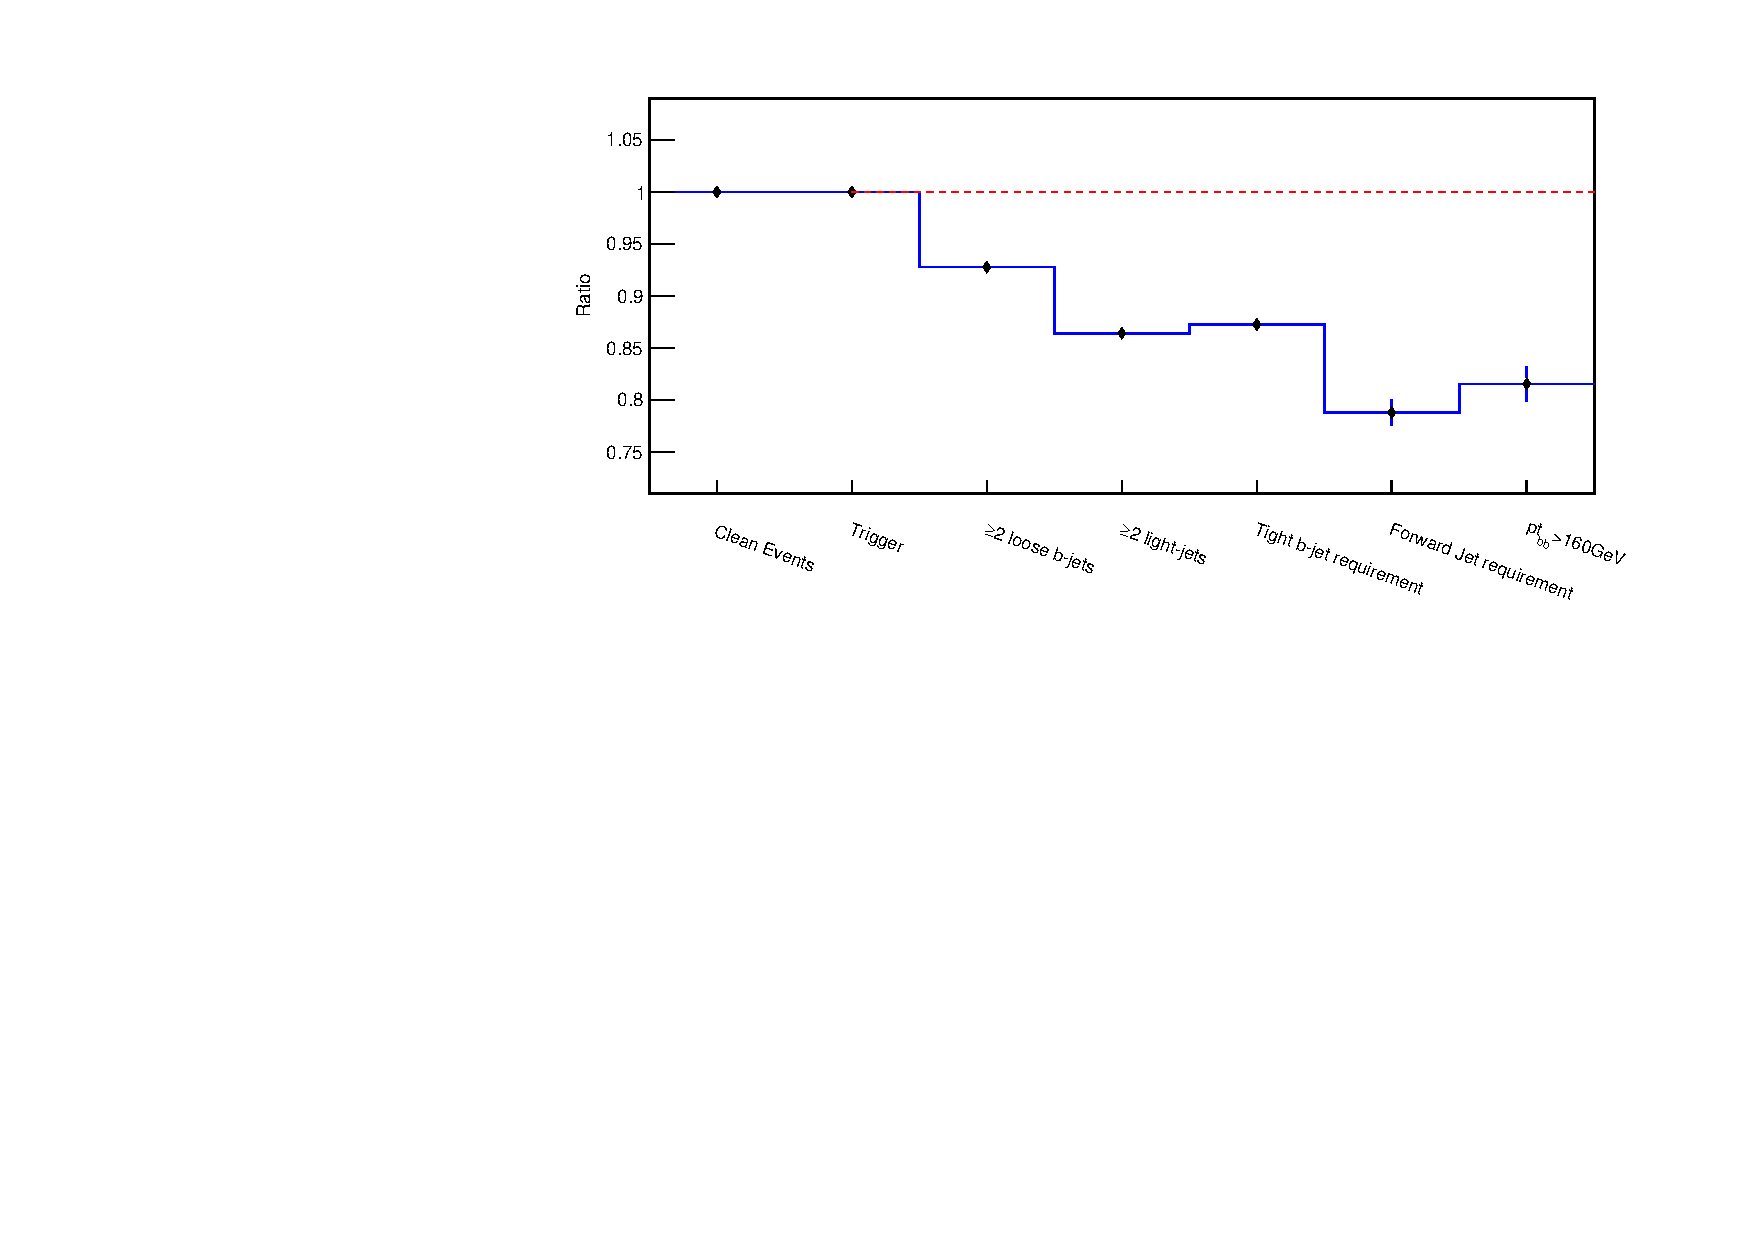
\includegraphics[width=0.75\linewidth]{MC_cutflow}
            \caption[\VBFHBB\ Cutflow ratio for Monte-Carlo simulation]{Ratio of the online event count over the offline event count for the Monte-Carlo simulations.}
            \label{f:cutflowMC}
        \end{figure}

    The online performance has fewer events than the offline for all points in the cutflow, and overall produces $\sim82\%$ of the total signal events. There are three distinct jumps in the cutflow ratio: at the cuts on the \textit{loose} \bjets, light-jets and the forward jet requirement, of~$\sim7\%$ each. As shown in Figure \ref{fig:MC:bjetefficiency}, online \btag\ is $\sim93\%$ as efficient as the offline \btag\ in Monte-Carlo simulations. When considering tagging two distinct \bjets, any difference in efficiency is squared. Given the difference in tagging rates, this would result in $\sim86\%$ tagging efficiency for two \bjets, which is lower than shown in the cutflow. As shown for the leading \bjet\ in Section \ref{OP:leadingb}, the offline jet is typically higher in \pt than the corresponding online jet. However the difference is small, $\sim2\%$, so any effect on the cutflow should not be very pronounced.

    The $\sim7\%$ drop on the light jet requirement is unexpected, as the requirement was solely for 2 non-\bjets\ with \pt$>20$~GeV. Given the points above with respect to the \pt difference between online and offline, this drop should not be so severe. The fact the \pt cuts on the light jets were so low also suggests an anomalous result, as such a cut should not contribute a significant reduction in either online or offline events.

    Following the drop for the light-jet cut, there is an unexpected increase in the online ratio following the tight \btagging\ cut. As highlighted, the tagging efficiency was worse for online than offline, so any requirement for a tagged \bjet\ would be expected to produce a decrease in the online event count, relative to the offline count. Perhaps spuriously, the cutflow at this point corresponds to the $86\%$ figure expected given the relative tagging efficiency for two \bjets.

    The final drop occurs following the requirement for a high \pt forward jet. Figure \ref{fig:O:leadingnonbptslice} shows that for non-\bjets\ in the forward region of the detector, the \pt of the offline jet is consistently higher than the online $p_\text{T}$. This difference would result in a drop in the online events, with fewer jets passing the threshold \pt cut compared to the offline events.

    For the Monte-Carlo events, while the individual steps of the cutflow show some unusual results, the overall effect was an 18\% reduction in the number of events that passed the \VBFHBB\, cuts.

    \subsection{Data}
        \begin{figure}[h]
            \centering
            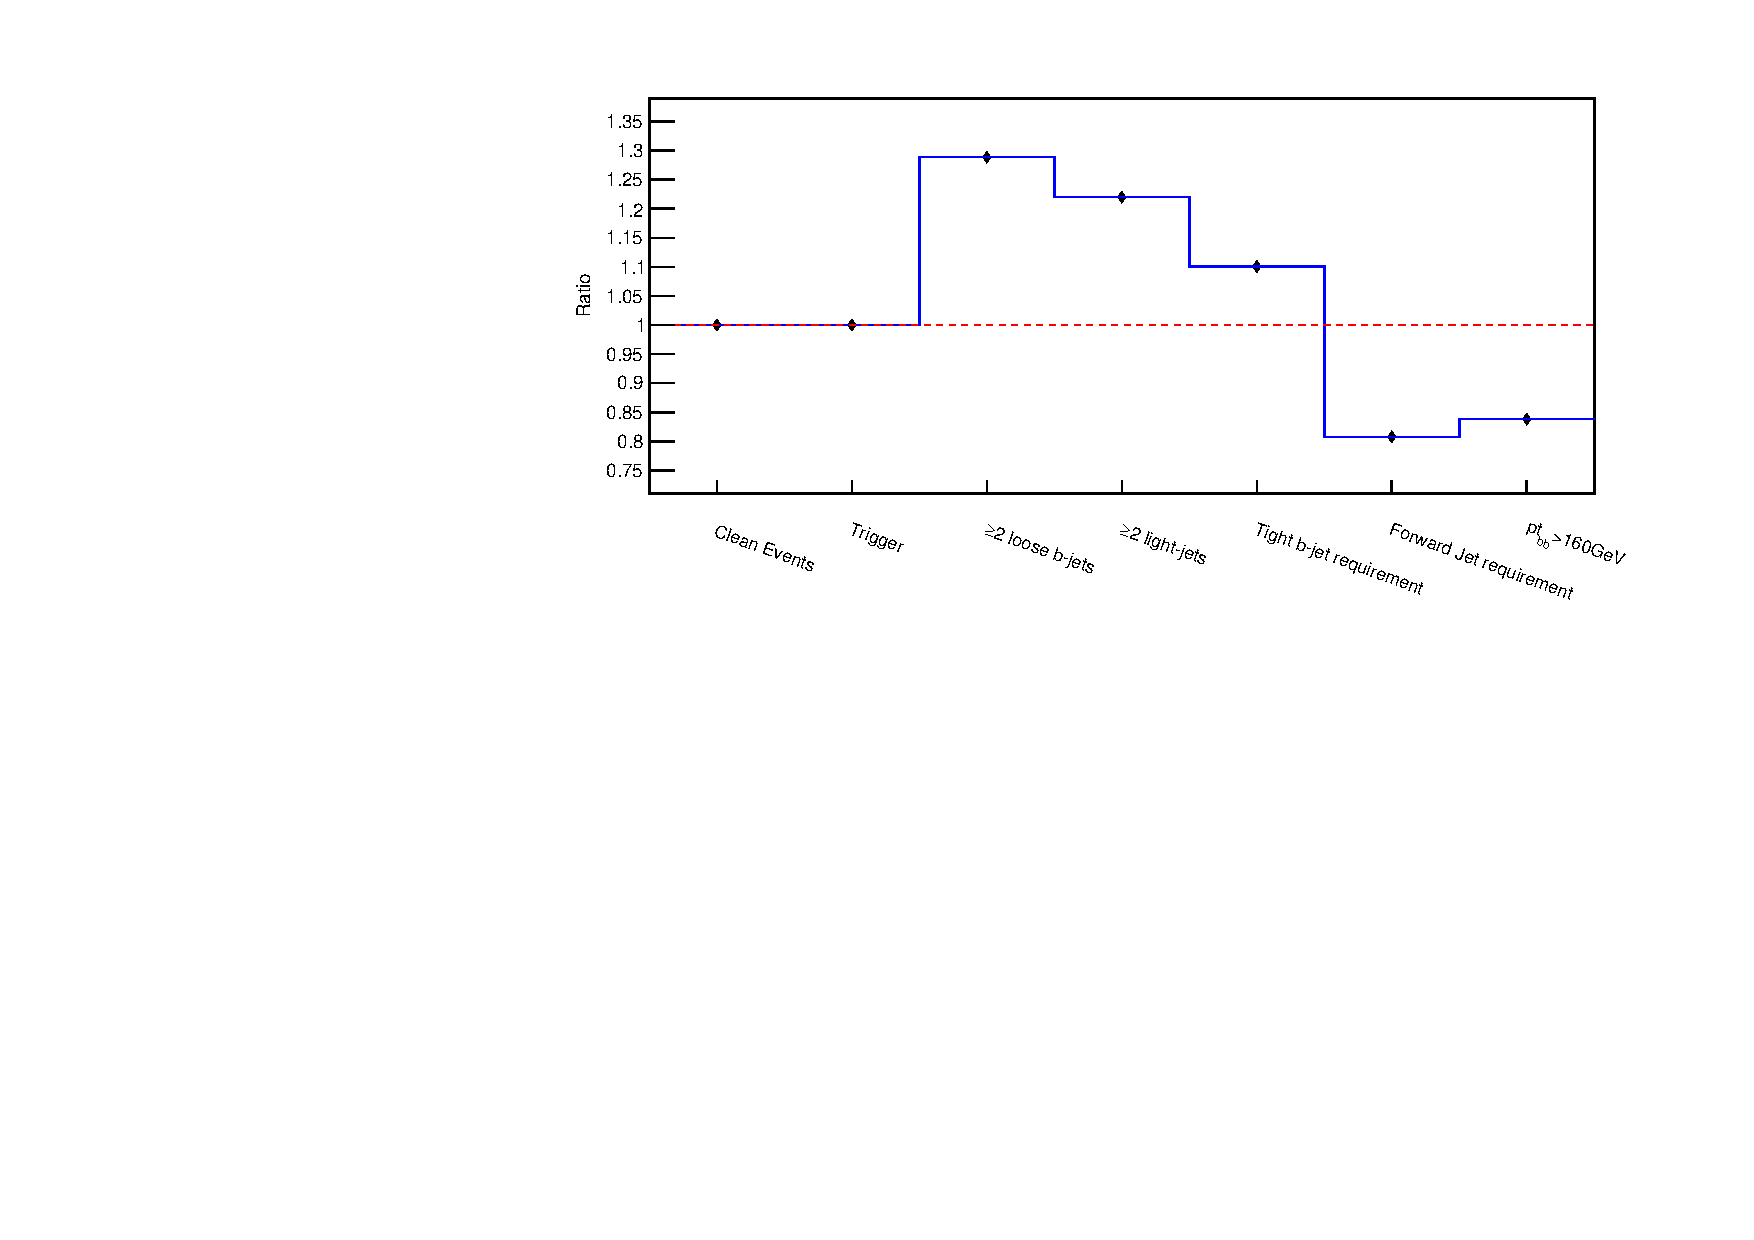
\includegraphics[width=0.75\linewidth]{D_cutflow}
            \caption[\VBFHBB\ Cutflow ratio for data]{Ratio of the online event count over the offline event count for the data.}
            \label{f:cutflowD}
        \end{figure}

    The cutflow performance in data shown in Figure \ref{f:cutflowD} does not show the online event count being consistently lower than offline as demonstrated for the Monte-Carlo simulations in Figure \ref{f:cutflowMC}. The overall effect of the cutflow for data described by Table \ref{t:cutflow} is a reduction in online events compared to offline events of $\sim84\%$.

    The first step shows a 25\% increase in the number of events passing the loose \bjets\ cut online compared to offline. If the \btag\ is assumed to perform in the same way for data as for Monte-Carlo simulations, in that the differences between the MV2c10 and MV2c20 algorithms shown for the Monte-Carlo simulations (Figure \ref{fig:MC:bjetefficiency}) are consistent, a decrease would be expected after this cut, rather than an increase. However, the trigger applied to the data requires one tight \bjet, so simple extrapolations of efficiency differences between online and offline are not straightforward to understand. Additionally, the trigger required a \bjet\ with \pt$>80$~GeV and the loose selection required \bjets $>70$~GeV, meaning the offline results are skewed by trigger turn-on curves and different jet energy scale requirements.

    Given the trigger selections (The \bjet\ identification and the \pt thresholds) are applied only in data, it is difficult to compare the relative normalisation of data and Monte-Carlo until the forward jet requirement is imposed (At which point all offline selections are in the plateau of the jet turn-on curve). After this requirement, both the data and Monte-Carlo show a ratio of $\sim0.8$.

    \subsection{Summary of Cutflow Comparison for the \VBFHBB\ events}

    The final reduction in online event count relative to the offline event count for the Monte-Carlo simulations was $\sim82\%$ of the offline event count, and $\sim84\%$  for the data. The results from individual steps in the cutflow are not supported by the results of Chapter \ref{c:OP}, but these overall results, which are broadly consistent for both data and Monte-Carlo, are supported by the expected decrease in efficiency as a result of the diffent \btag\ algorithms. Looking only at the overall reduction at the final states suggests that future analyses may be able to apply TLA to the \VBFHBB\ channel to increase the final event yield.

    With an average $\sim83\%$ reduction in event rate for the channel, usage of TLA at a rate of $2$~kHz as described in Ref. \cite{tla} and Section \ref{t:tla}, would result in an increase in output events of $\sim66\%$ compared to a standard offline analysis. This may not result in an increase in the signal from the analysis, but given the reduced bandwidth requirements of TLA, the trigger selections could be loosened to increase the signal efficiency. Analysis of this is beyond the scope of this dissertation.

    This value is an estimate; there is additional computational cost involved with storing and computing the quantities required for TLA \VBFHBB\ analysis, such as the increased event size mentioned in Section \ref{obp:beff} as a result of storing the \btag\ training quantities. Carrying out a rate analysis, to ensure the TLA can be applied in the \VBFHBB\ channel without decreasing the rate increase down to the point the final TLA event count is no longer an improvement, is a necessary step before approving TLA, but is beyond the scope of this dissertation.

\newpage
\section{Specific Jet Feature Distributions}
\label{k:jets}

    While the previous chapter showed that the \bjets\ and non-\bjets\ had slight differences that could be rectified for future analyses, the behaviour of those jets is sufficiently similar that plots of the kinematic quantities of the \VBFHBB\ jets can be made. The plots have been normalised to equal sums of weights to permit shape comparisons.

    \begin{table}[h]
        \caption[Signal/Background definition \mbb values]{\mbb bins defining an event as signal or background, along with the data source for the quantities.}
        \label{t:signalback}
        \medskip
        \centering
        \begin{tabular}{ccc}\toprule
            Designation & \mbb range / GeV & Sample \\\midrule
            Background (Lower) & \mbb<$100$ & Data \\
            Signal & $100<$\mbb$<140$ & Monte-Carlo \\
            Background (Upper) &  $140<$\mbb & Data \\
            \bottomrule
        \end{tabular}
    \end{table}

    These plots are presented in signal and background regions, as defined by the \mbb value as shown in Table \ref{t:signalback}. The signal was plotted only using the Monte-Carlo simulation while the background regions were taken from data events. The kinematic quantities for leading \bjet\ and leading non-\bjet\ of the \VBFHBB\ event are plotted for both the online and offline objects. The \pt distributions are shown in Figures \ref{f:ptb1} and \ref{f:ptj1} respectively, while the pseudorapidity plots are shown in Figure \ref{f:etab1} and \ref{f:etaj1}.

        \begin{figure}[h]
            \centering

            \begin{minipage}[h]{0.48\linewidth}
                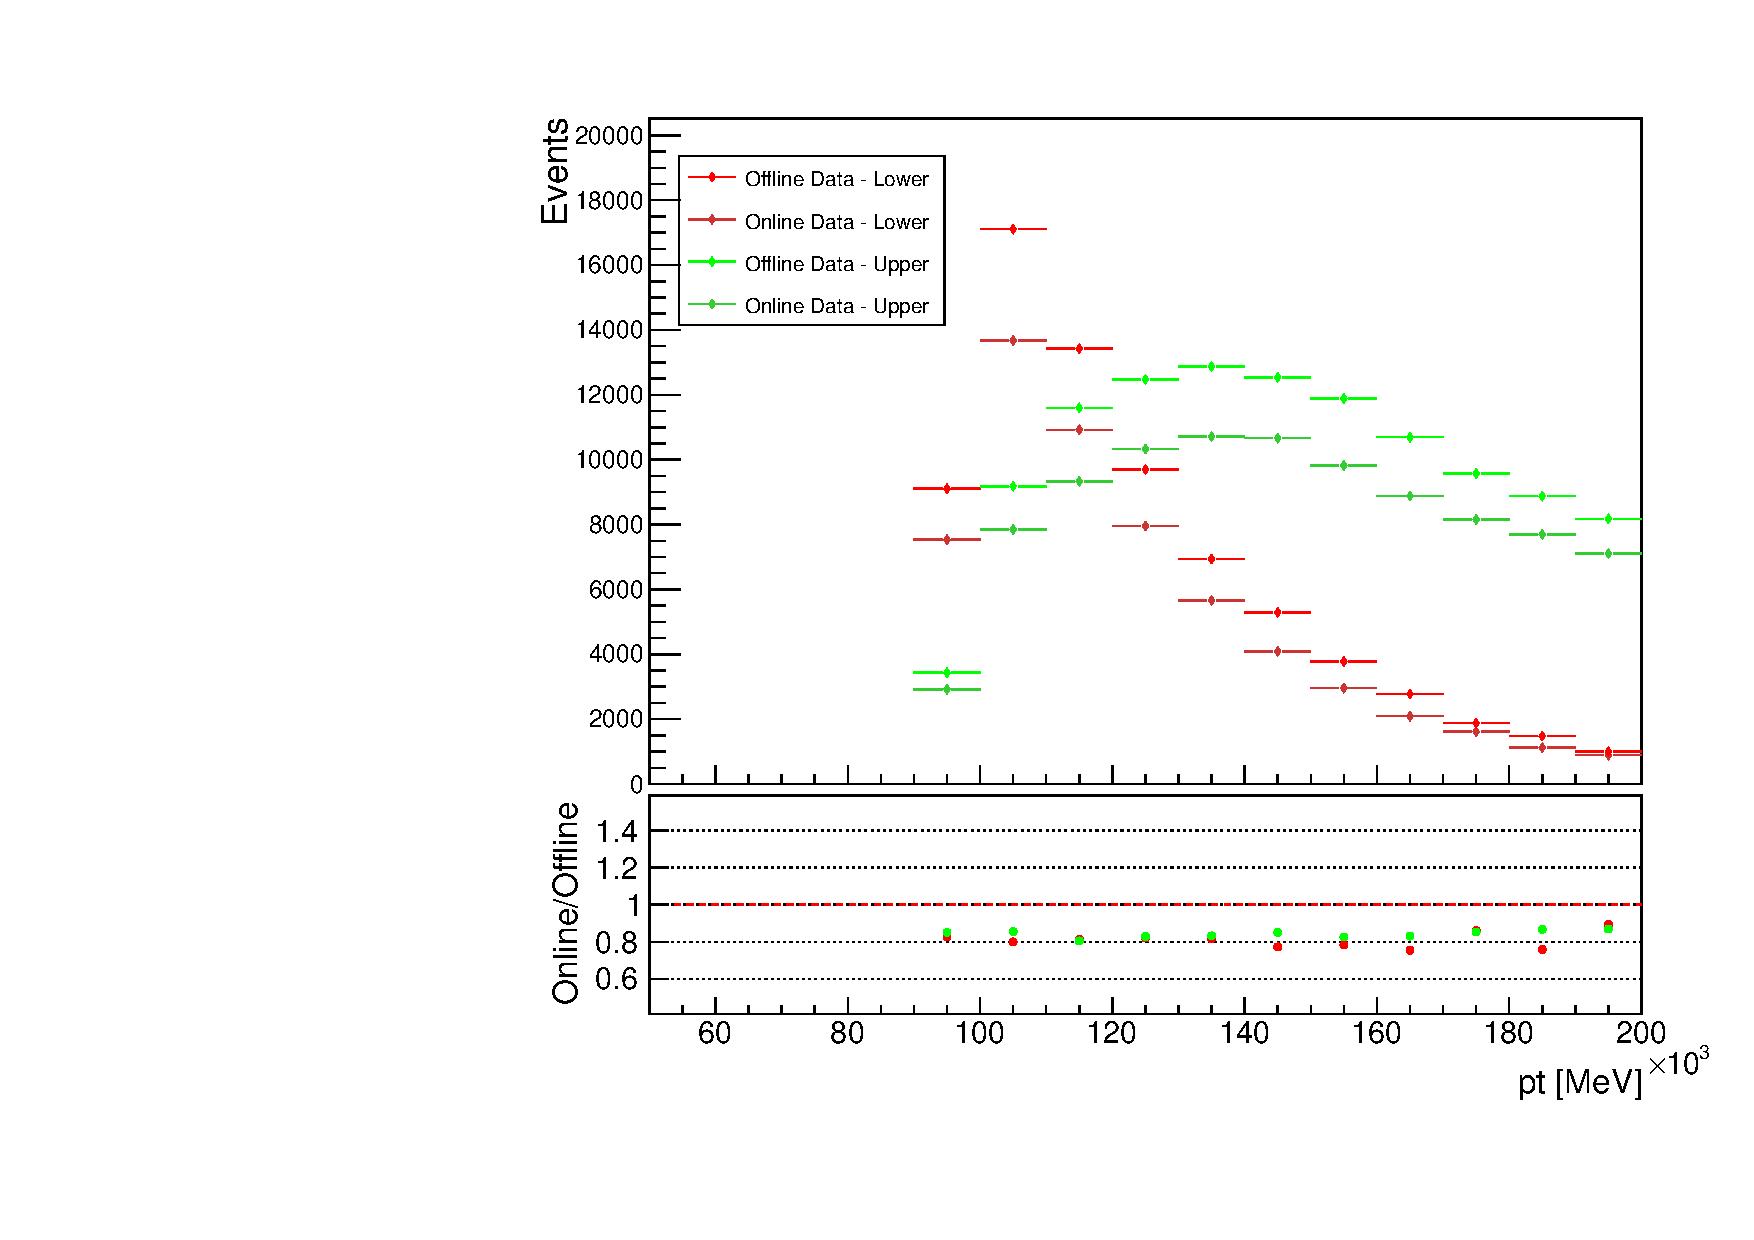
\includegraphics[width=1\linewidth]{pt_bJet1_data_}
            \end{minipage}
            \quad
            \begin{minipage}[h]{0.48\linewidth}
                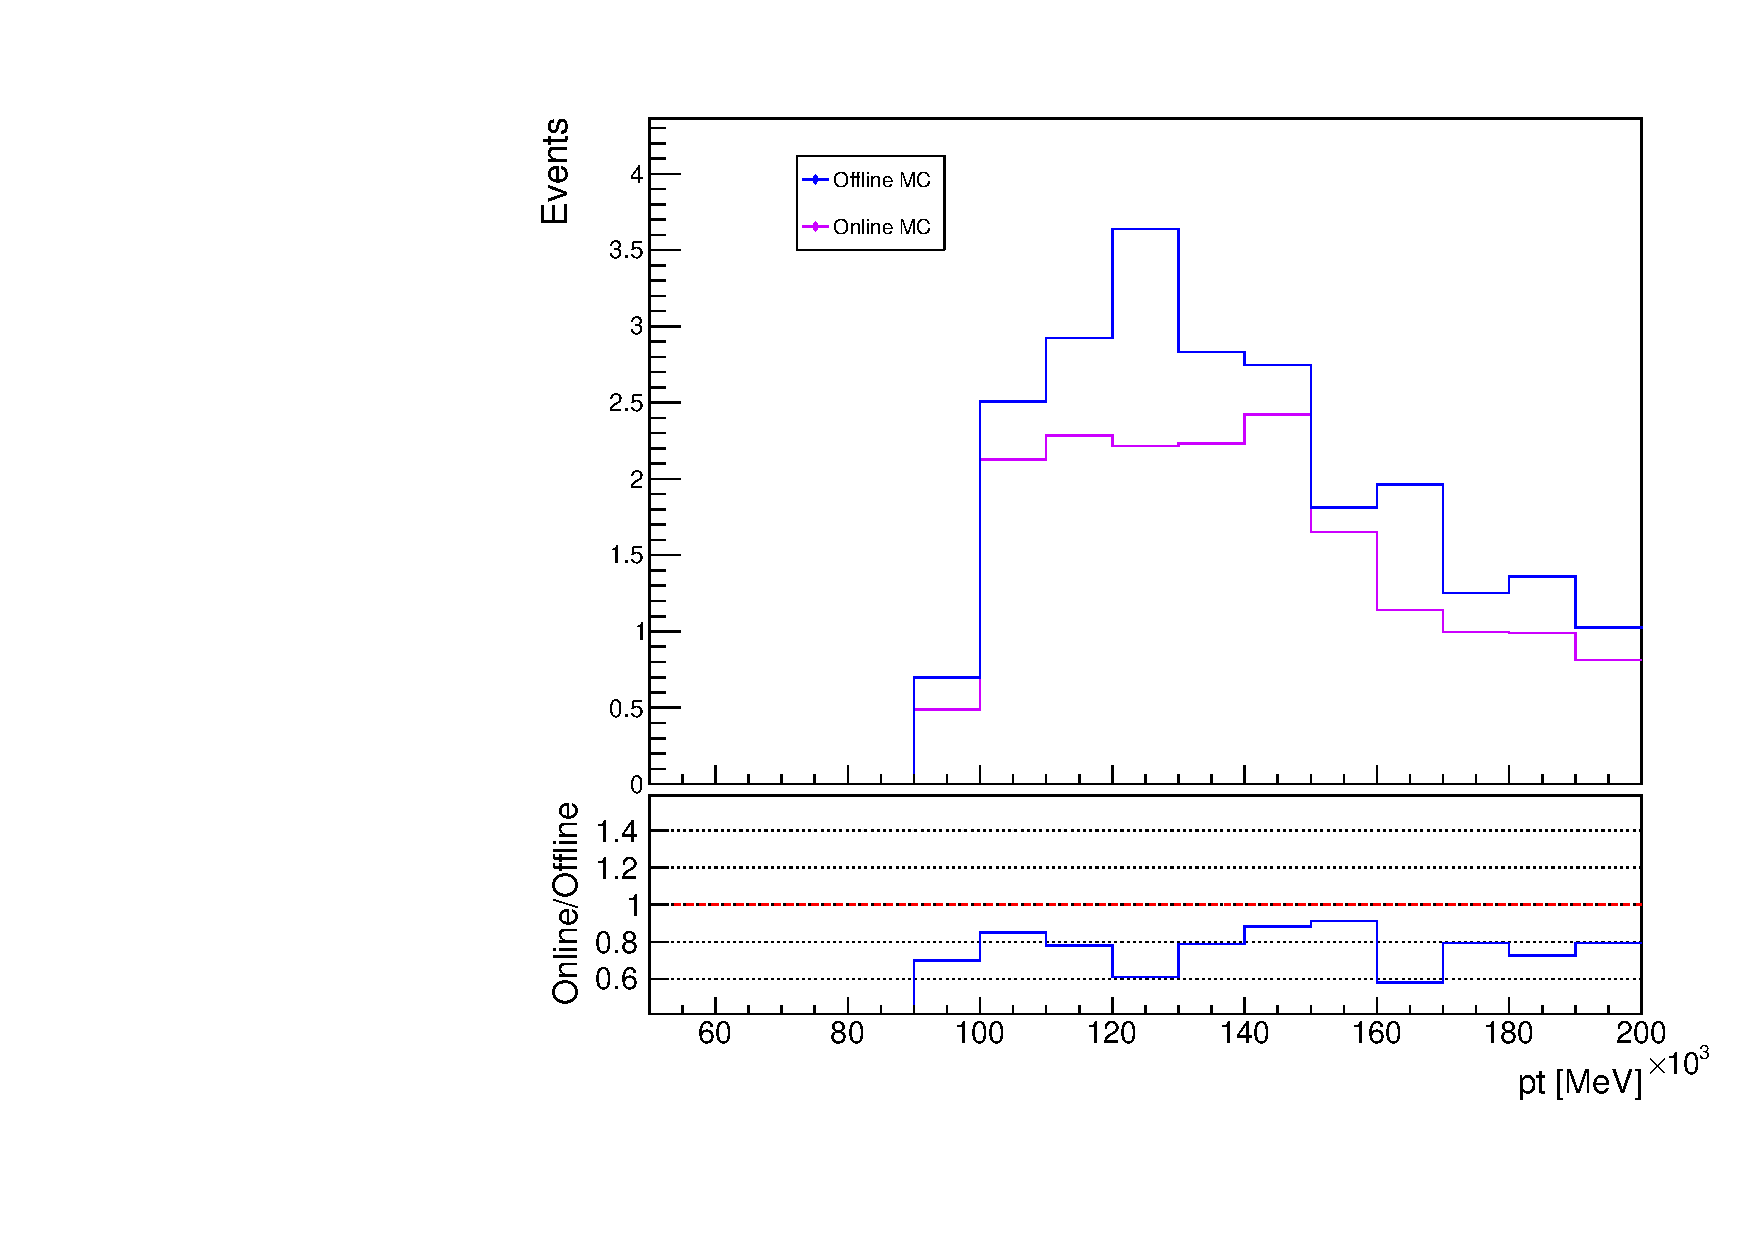
\includegraphics[width=1\linewidth]{pt_bJet1_mc_}
            \end{minipage}
            \caption[\pt distribution of the leading \bjet\ of the \VBFHBB\ event]{\pt distribution of the leading \bjet\ of the \VBFHBB\ event, plotted for both the backgroud data regions in the left panel and Monte-Carlo signal events in the right panel.}
            \label{f:ptb1}
        \end{figure}

        \begin{figure}[h]
            \centering

            \begin{minipage}[h]{0.48\linewidth}
                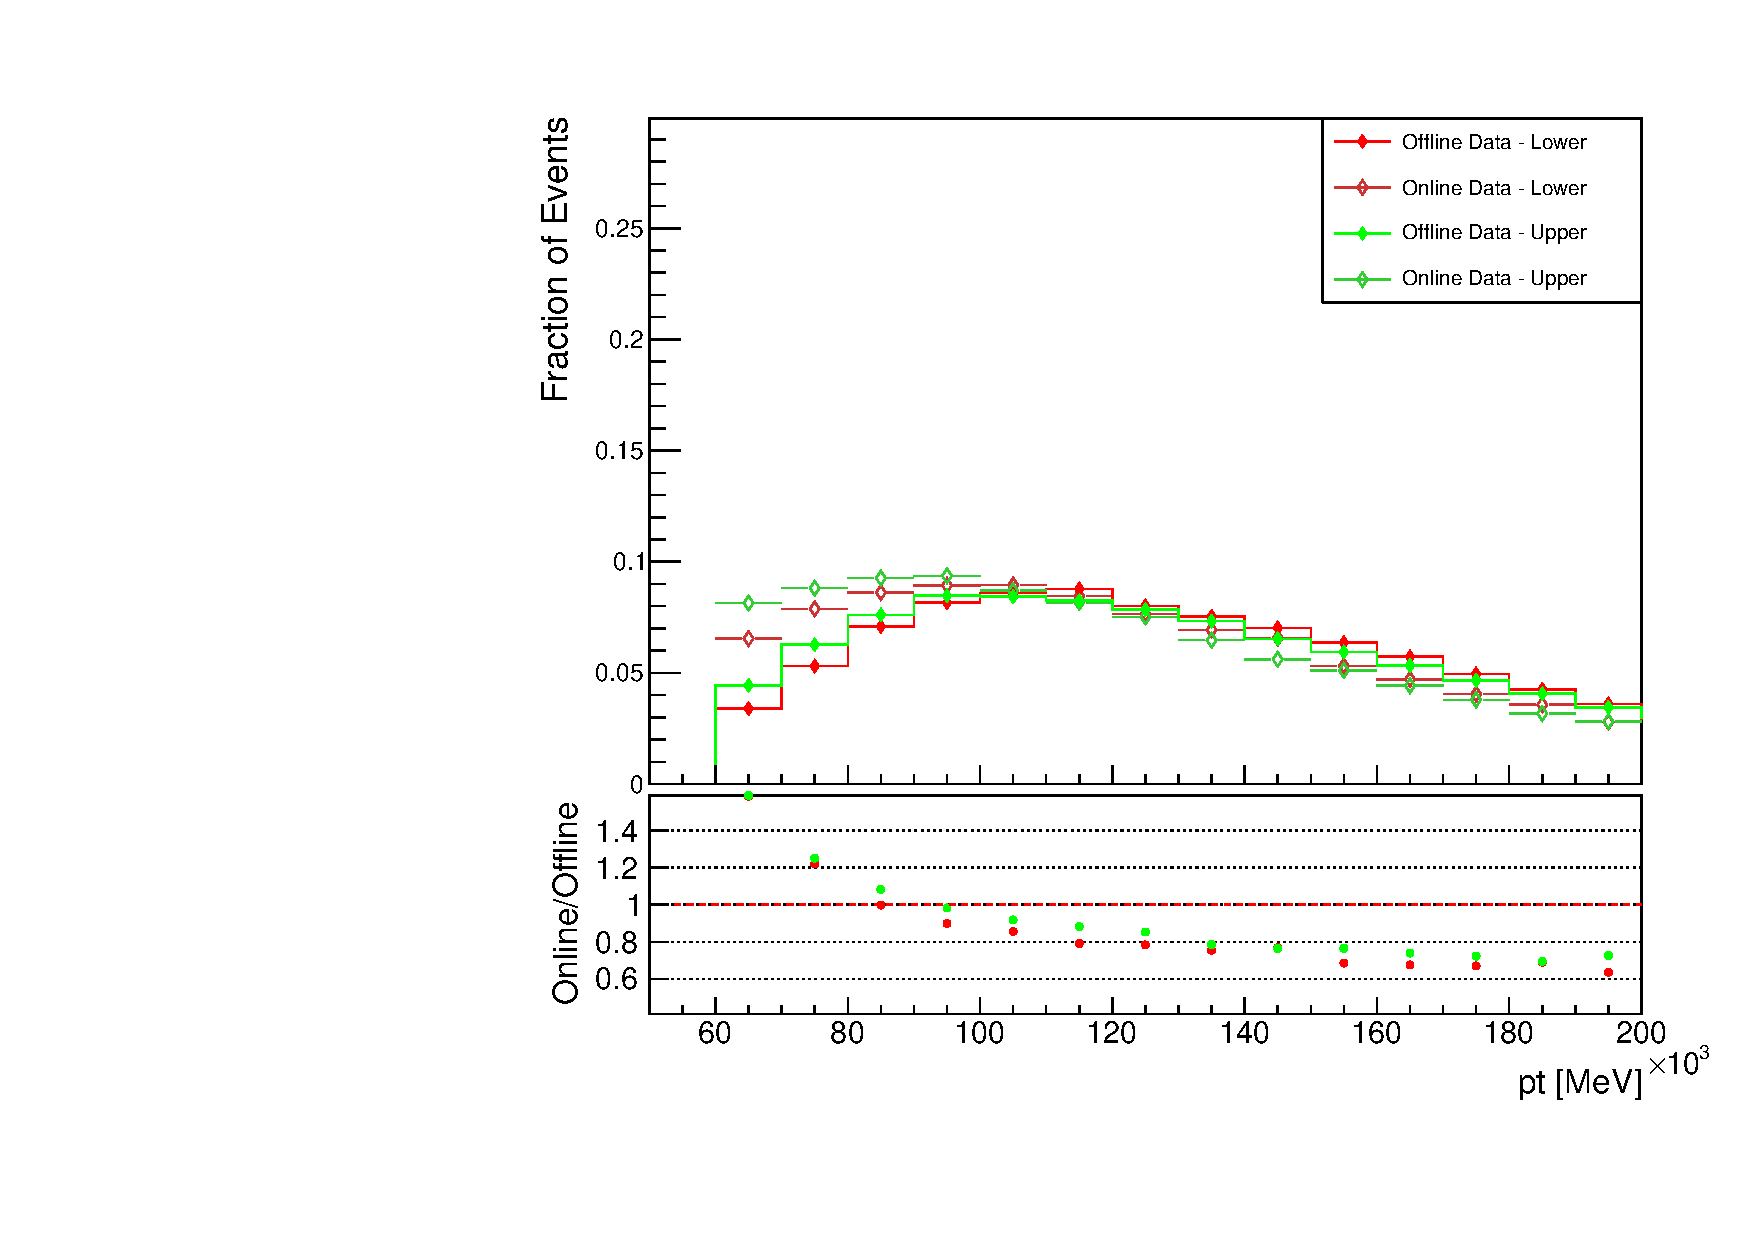
\includegraphics[width=1\linewidth]{pt_lJet1_data_}
            \end{minipage}
            \quad
            \begin{minipage}[h]{0.48\linewidth}
                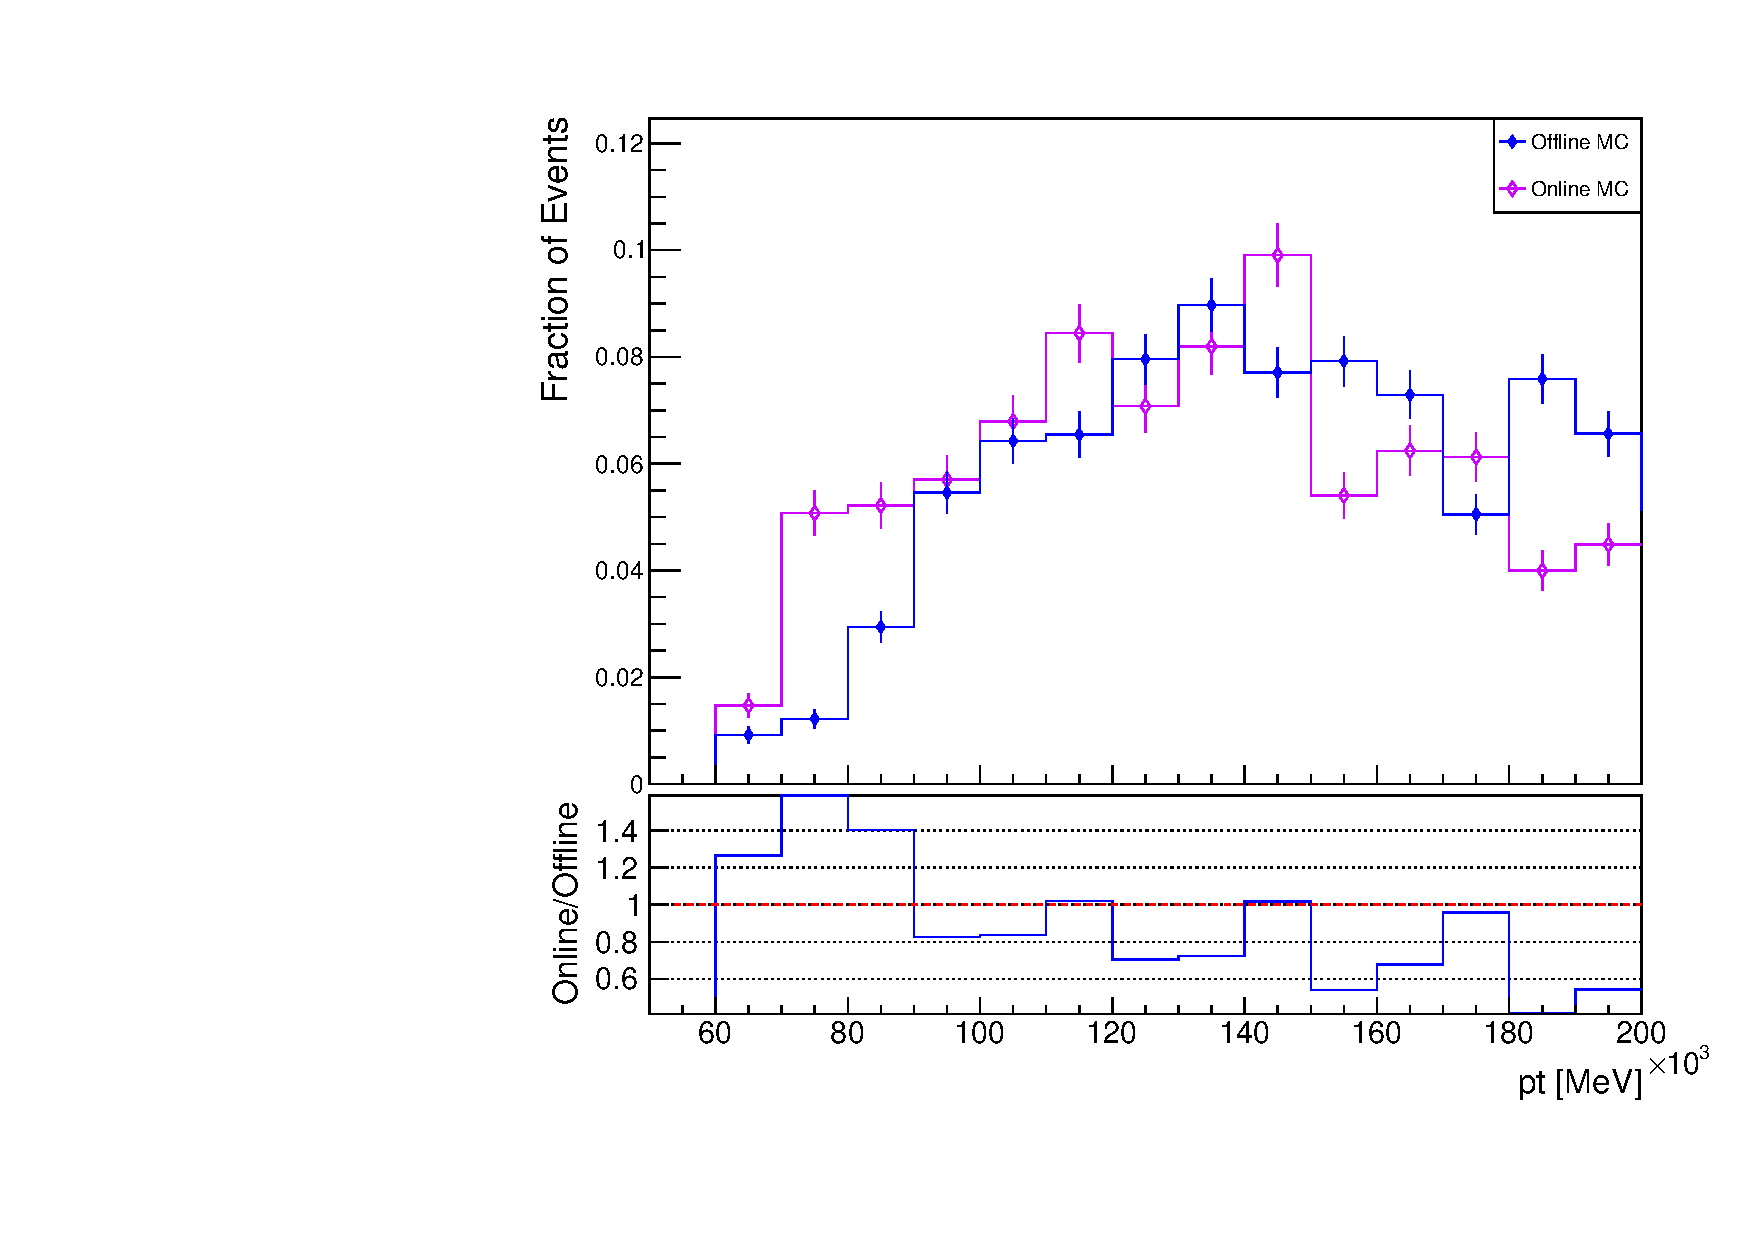
\includegraphics[width=1\linewidth]{pt_lJet1_mc_}
            \end{minipage}
            \caption[\pt distribution of the leading non-\bjet\ of the \VBFHBB\ event]{\pt distribution of the leading non-\bjet\ of the \VBFHBB\ event, plotted for both the backgroud data regions in the left panel and Monte-Carlo signal events in the right panel.}
            \label{f:ptj1}
        \end{figure}

    The distribution of the \pt values for the leading \bjet\ shown in Figure \ref{f:ptb1} peaks at a higher value for the upper background region than the lower background region. This is a result of the \mbb sculpting the background distributions, as higher \mbb values will correlate with higher \bjet\ \pt values. For the background \pt plot of the leading non-\bjet, this sculpting is not seen as the \pt of the forward jet is not directly linked to the \mbb of the event. For both the leading \bjet\ and the leading non-\bjet\, the online and offline distributions are similarly shaped for each of the defined \mbb regions.

    For the leading \bjet, the ratio of the online to the offline events shown in Figure \ref{f:ptb1} is flat in both the upper and lower background regions, and has a value of $\sim0.8$. This value is consistent with the expected decrease in the online event count shown in Figure \ref{f:cutflowD}. The Monte-Carlo signal plot shown in Figure \ref{f:ptb1}, the line is insufficiently clear to make a firm statement but the ratio values are distributed around $0.8$. For the leading non-\bjet, the behaviour of the online/offline ratio is more complex, as shown by the distinct curve in the left panel of Figure \ref{f:ptj1}. The online jets show a bias towards low \pt compared to the offline jets in both the upper and lower background regions, along with in the signal region. The relative ratio of the online and offline jets is affected by this, flattening out at a lower value of $\sim0.7$ than the expected $0.8$ in both the background regions. This bias towards lower \pt events was seen in Figure \ref{fig:O:leadingnonbpt} in the previous chapter showing the \dptpt distribution for the leading non-\bjet. Figure \ref{fig:O:leadingnonbpt} showed a large number of data jets with offline transverse momentum $50<$ \pt$<90$~GeV which had a \dptpt value between 0.1 and 0.2, indicating that for this region the offline \pt was significantly larger than the online. This observation is consistent with the left panel of Figure \ref{f:ptj1}, as it suggests there will more online jets with $50<$ \pt$<80$~GeV than offline jets in the data, accounting for the shift in the distribution peaks. For the signal plot, Figure \ref{fig:O:leadingnonbpt} did not show such a pronounced discrepancy for the Monte-Carlo jets, only a slight increase of \dptpt values around 0.1 for this low \pt region, so such a shift is not absolutely expected for the signal region. In addition, as for the leading \bjet, a clear statement on the ratio of the Monte-Carlo events cannot be made, but the curve broadly follows the background ratios.

    While there are differences between the signal and background regions and the small effects at low \pt in the leading non-\bjets, for the complete \pt distributions of leading \bjet\ and most of the distribution for the leading non-\bjet\ the offline jets performed the same as the online jets. This suggests that the online jet objects could be used in a TLA without any major effects on the outcome.

    The plots for the same leading jet objects against $\eta$ show the expected features for \VBFHBB\ jets. Figure \ref{f:etab1} shows the pseudorapidity ranges for the \bjet\ confined to the central region of the detector where \btag\ is operational. The $\eta$ plot for the leading non-\bjet\ displays spikes of events with $|\eta|\sim3$, which is expected given the requirements for a forward jet passing a \pt cut covered in Section \ref{es:as}. These features are present in both the signal and background regions.

    \begin{figure}[h]
        \centering

        \begin{minipage}[h]{0.48\linewidth}
            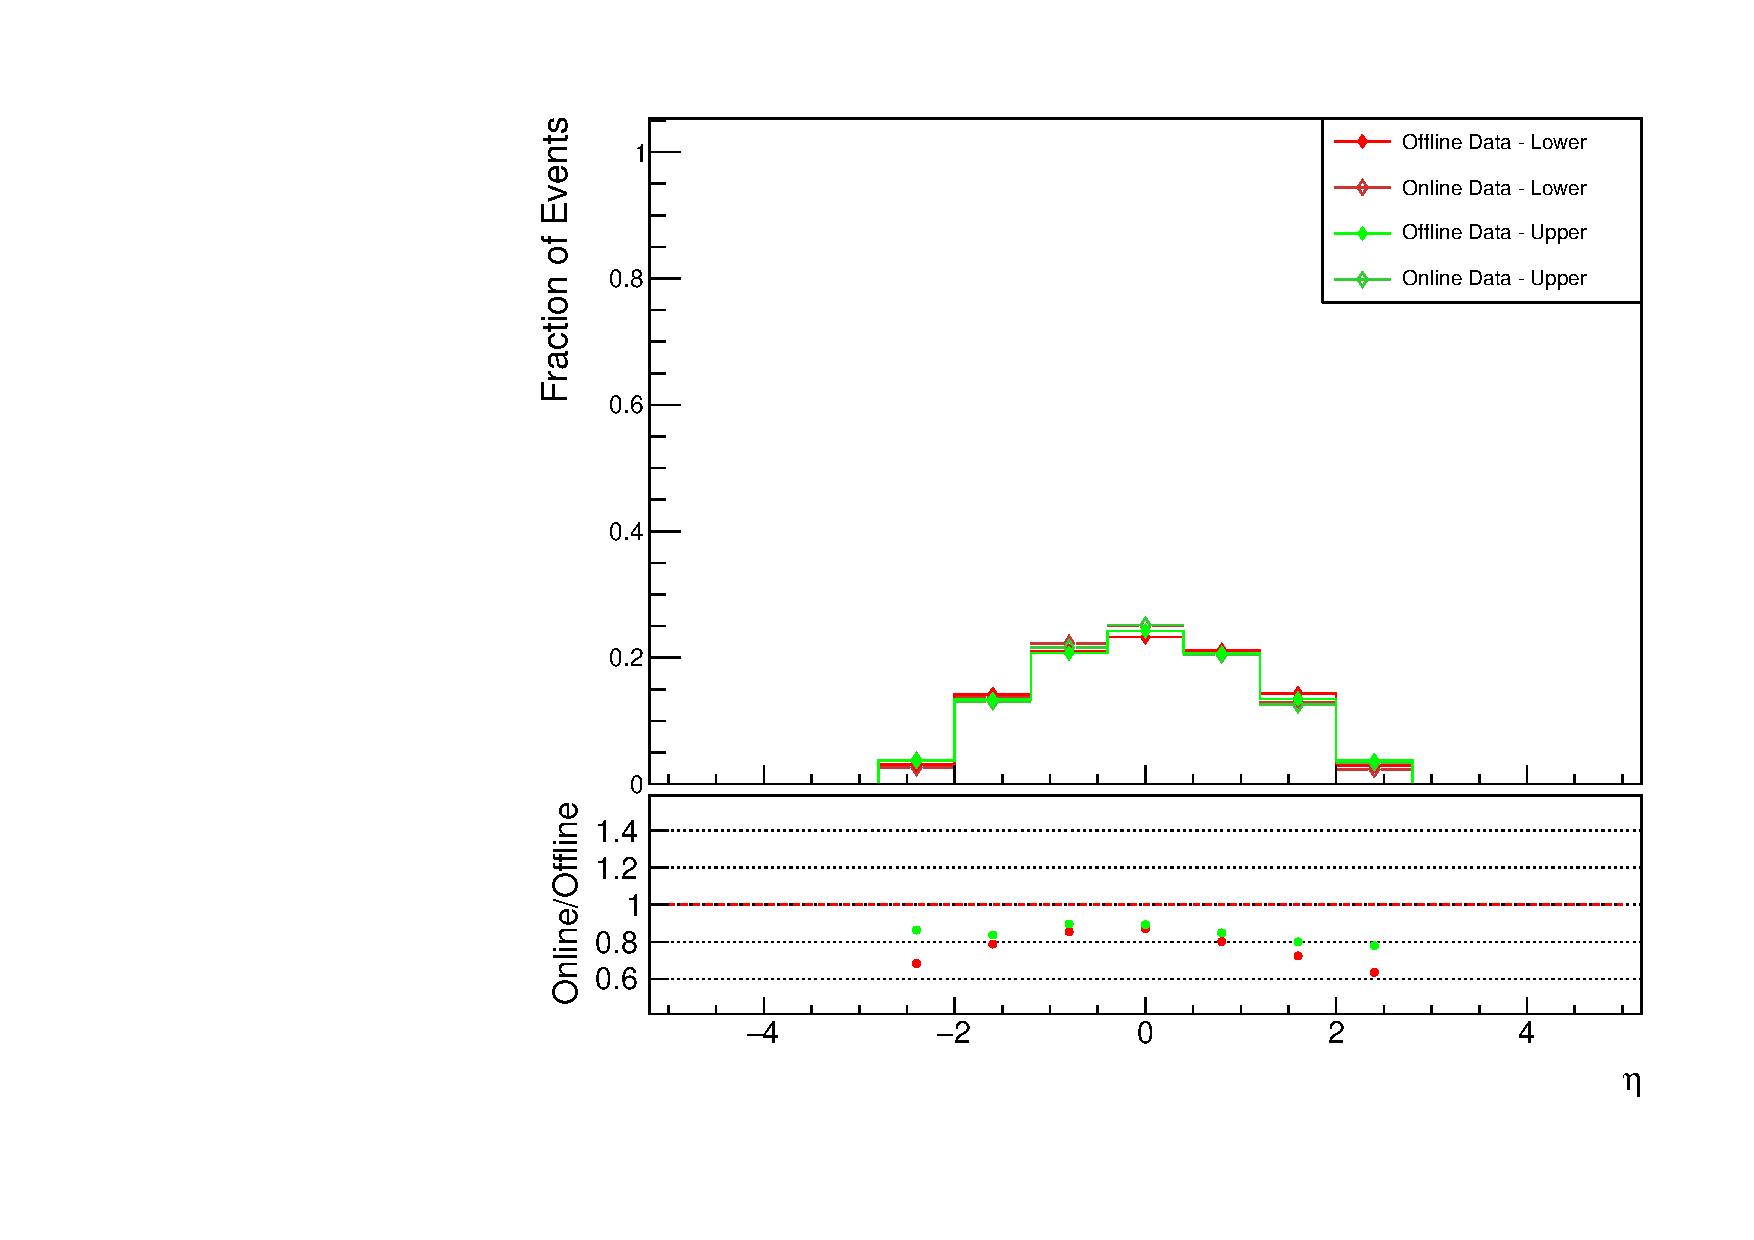
\includegraphics[width=1\linewidth]{eta_bJet1_data_}
        \end{minipage}
        \quad
        \begin{minipage}[h]{0.48\linewidth}
            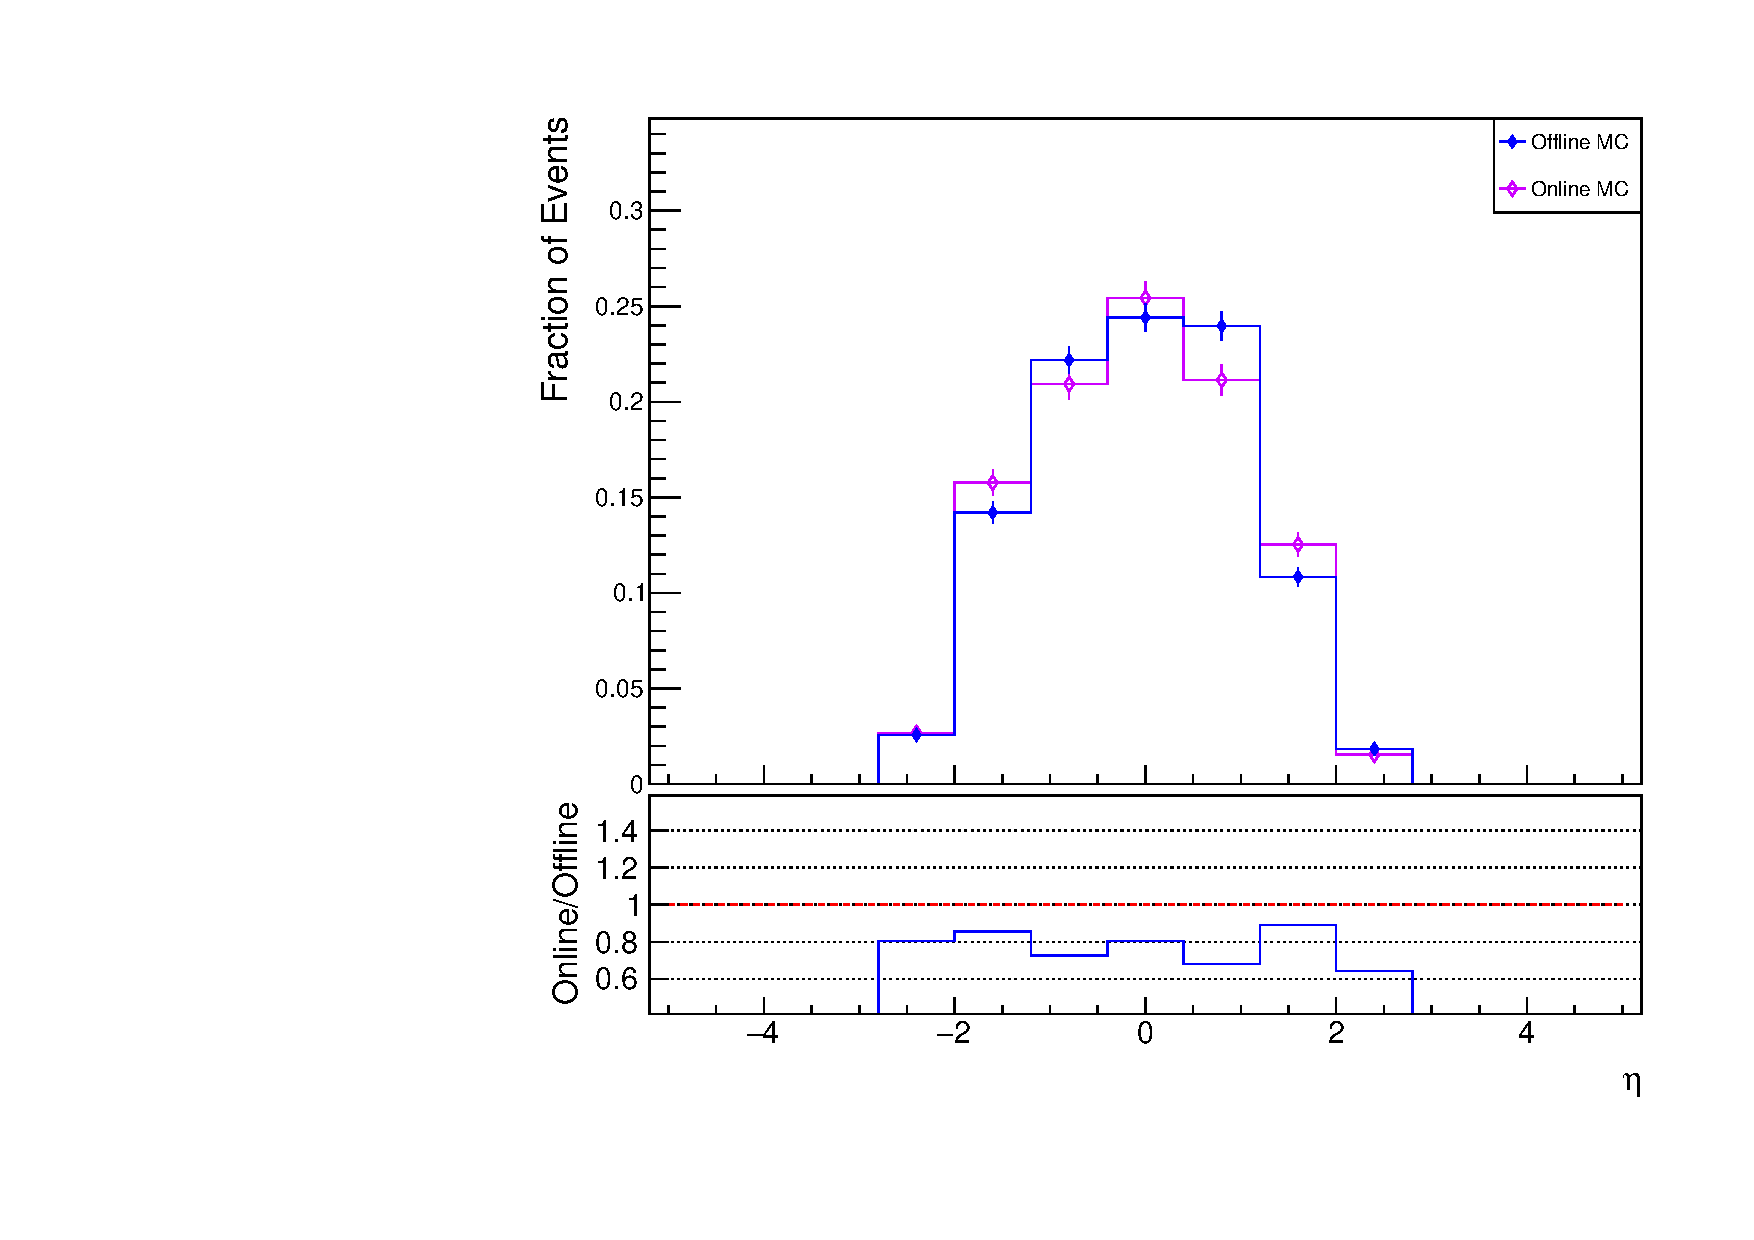
\includegraphics[width=1\linewidth]{eta_bJet1_mc_}
        \end{minipage}
        \caption[$\eta$ distribution of the leading \bjet\ of the \VBFHBB\ event]{$\eta$ distribution of the leading \bjet\ of the \VBFHBB\ event, plotted for both the background data regions in the left panel and Monte-Carlo signal events in the right panel.}
        \label{f:etab1}
    \end{figure}

    \begin{figure}[h]
        \centering
        \begin{minipage}[h]{0.48\linewidth}
            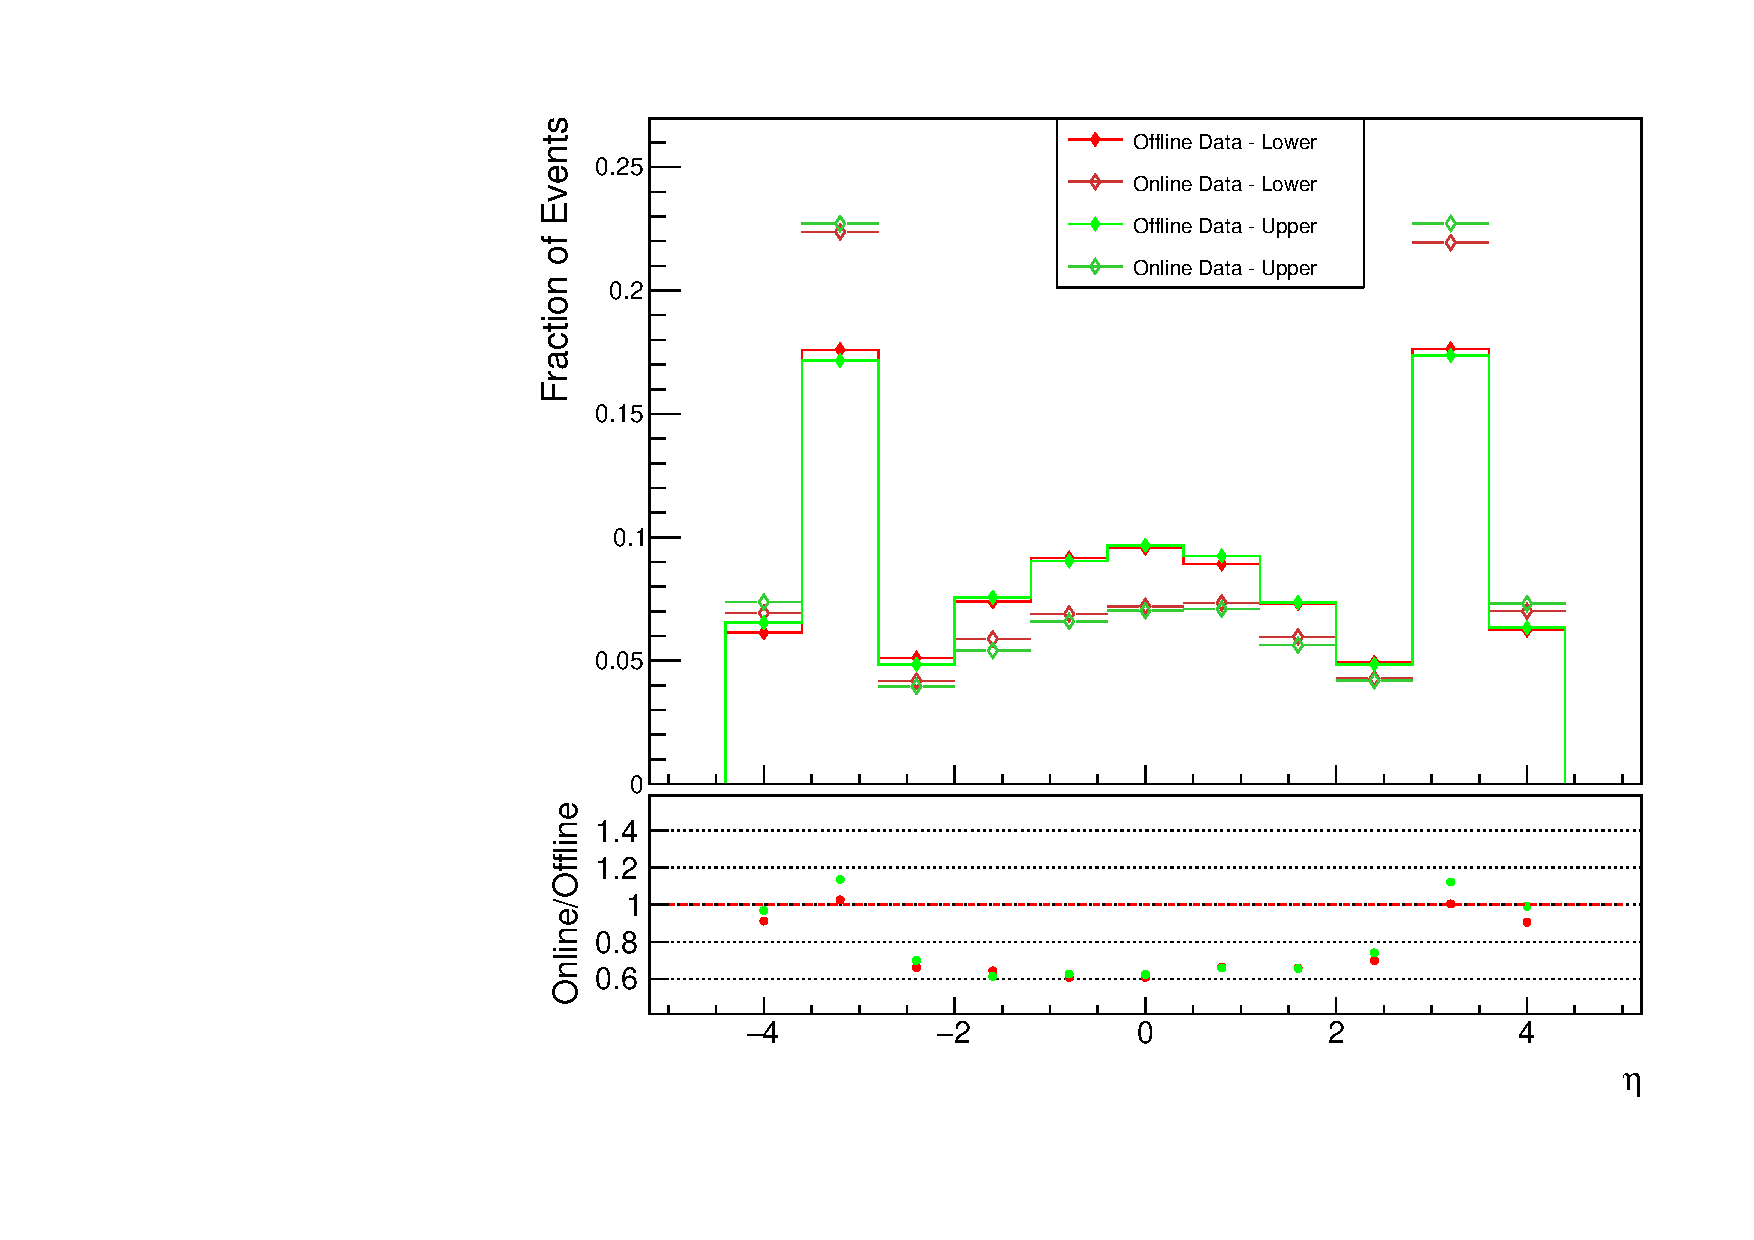
\includegraphics[width=1\linewidth]{eta_lJet1_data_}
        \end{minipage}
        \quad
        \begin{minipage}[h]{0.48\linewidth}
            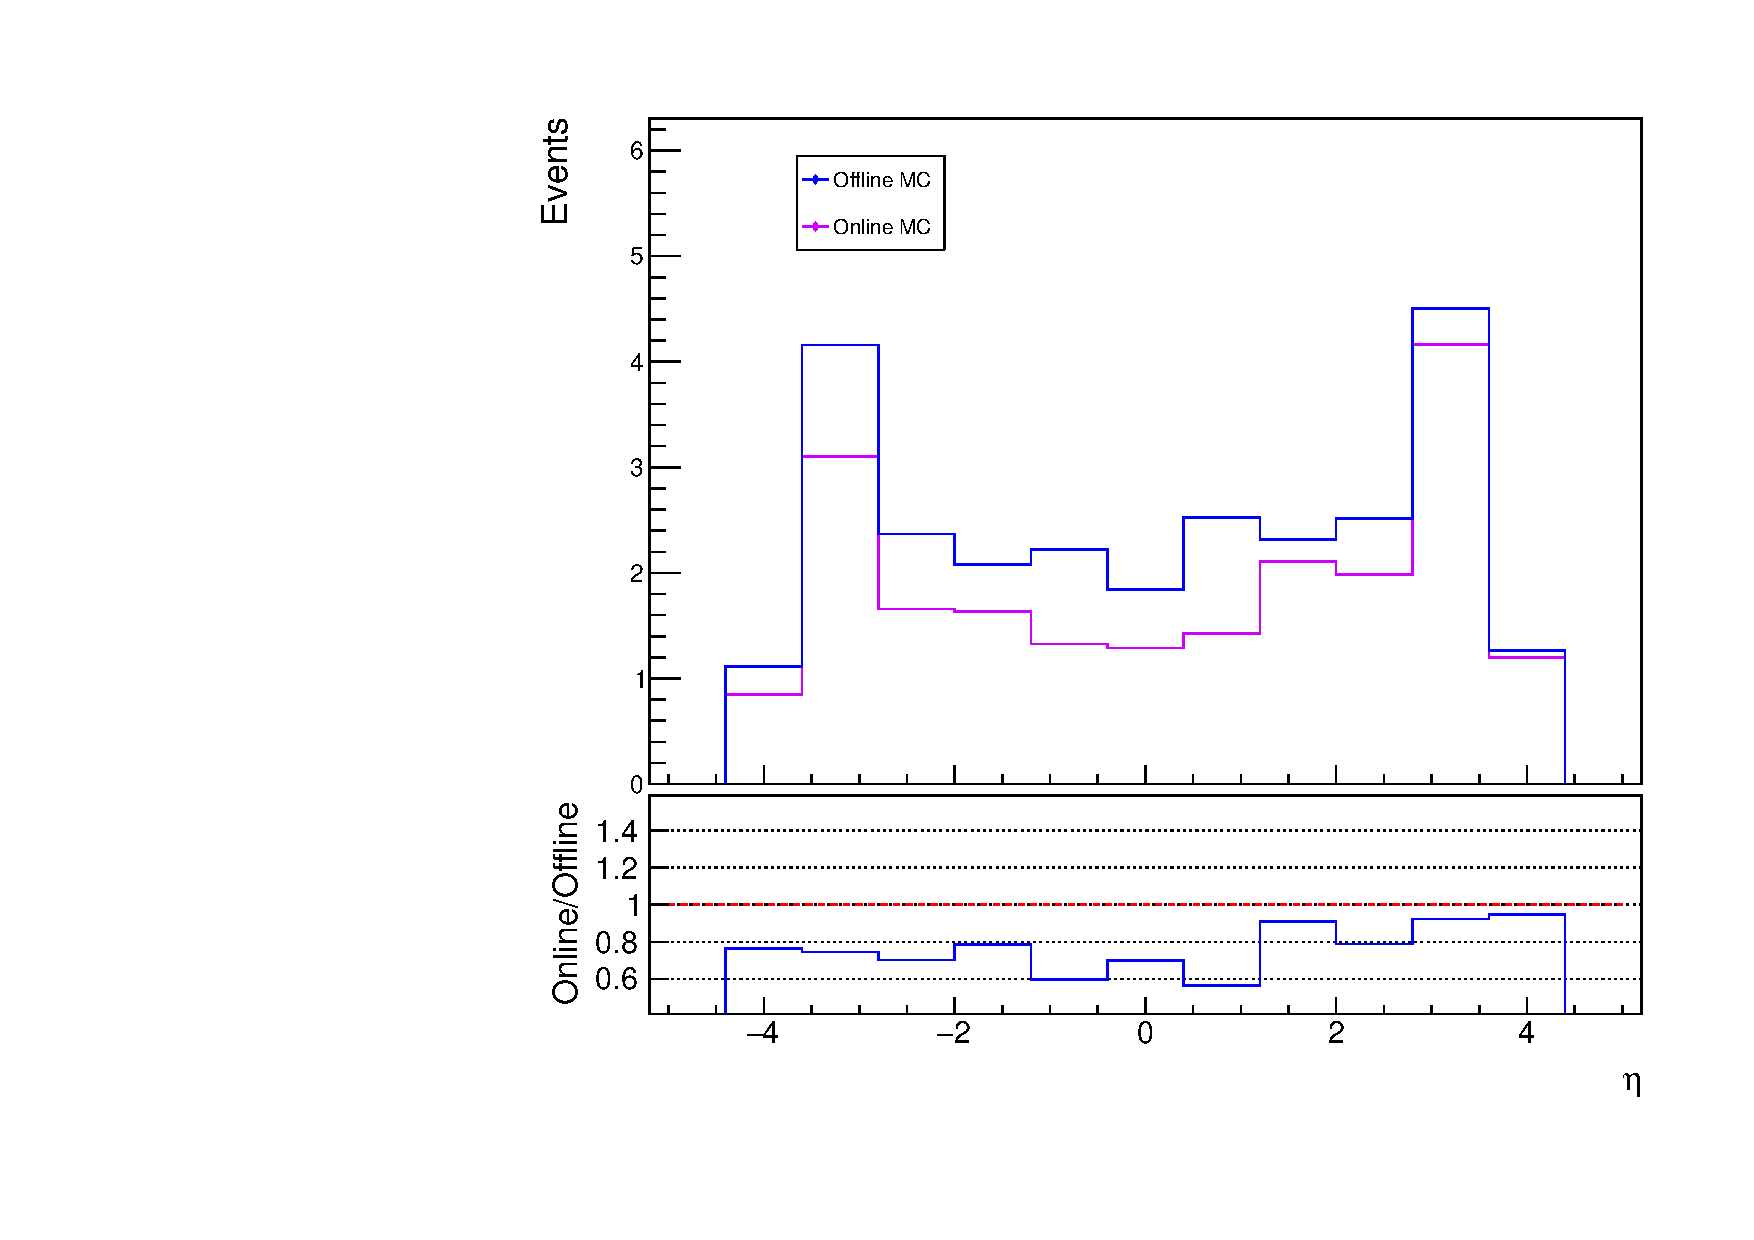
\includegraphics[width=1\linewidth]{eta_lJet1_mc_}
        \end{minipage}
        \caption[$\eta$ distribution of the leading non-\bjet\ of the \VBFHBB\ event]{$\eta$ distribution of the leading non-\bjet\ of the \VBFHBB\ event, plotted for both the background data regions in the left panel and Monte-Carlo signal events in the right panel.}
        \label{f:etaj1}
    \end{figure}

    The relative performance of online to offline shows some slight differences with respect to $\eta$. For the leading \bjet\ there is a noticeable peak in the ratio at $\eta=0$ for the lower signal region shown in Figure \ref{f:etab1}, however the upper signal region shows moderately consistent distribution around the expected $0.8$ value. The signal $\eta$ online/offline ratio has a larger degree of variation but is consistently around $\sim0.8$. For the leading non-\bjet\ shown in Figure \ref{f:etaj1} the ratio for the upper and lower background sectors is lower than expected in the central region of the detector, but increases in the forward regions. For the signal sector, the distribution suggests a slight increase of the ratio at the outer $\eta$ regions, but the difference is less pronounced than in the background regions.

    Overall, the behaviour of the leading jets of the \VBFHBB\ event was fairly consistent for online and offline in most phase space regions. The plots showed the distribution features expected for the variables and the differences associated with the \mbb bins, along with showing agreement with the reduction in event number for online events. The discrepancy in online behaviour relative to the offline for the low \pt leading non-\bjets\ can be explained by the observed differences in the non-\bjet\ objects explored in the previous Chapter, however the cause of the improved relative performance of the online objects in the forward regions for the leading non-\bjet\ are unknown. The upper background sector frequently had a higher ratio than the lower background sector, as shown across the entire \pt range in Figures \ref{f:ptb1} and \ref{f:ptj1}. These observations suggest a TLA using these objects would show little change in the overall behaviour, and if the calibration steps suggested in Section \ref{obp:jetsum} were applied, the differences in the online and offline behaviour may be removed.


\section{Kinematic quantities of the \VBFHBB\ event}

	Along with studying the kinematic quantities associated with single \VBFHBB\ jets, the kinematic properties of the jet pairs were compared for online and offline. For the non-\bjet\ pair, \ptjj and \mjj are plotted in Figures \ref{f:ptjj} and \ref{f:mjj}. Both of these variables are also training variables for the BDT used to refine the produced results (Appendix \ref{a:bdt}). Figure~\ref{f:ptbb} shows the \ptbb distribution and Figure~\ref{f:mbb} shows the \mbb distribution.

        \begin{figure}[h]
            \centering
            \begin{minipage}[h]{0.48\linewidth}
                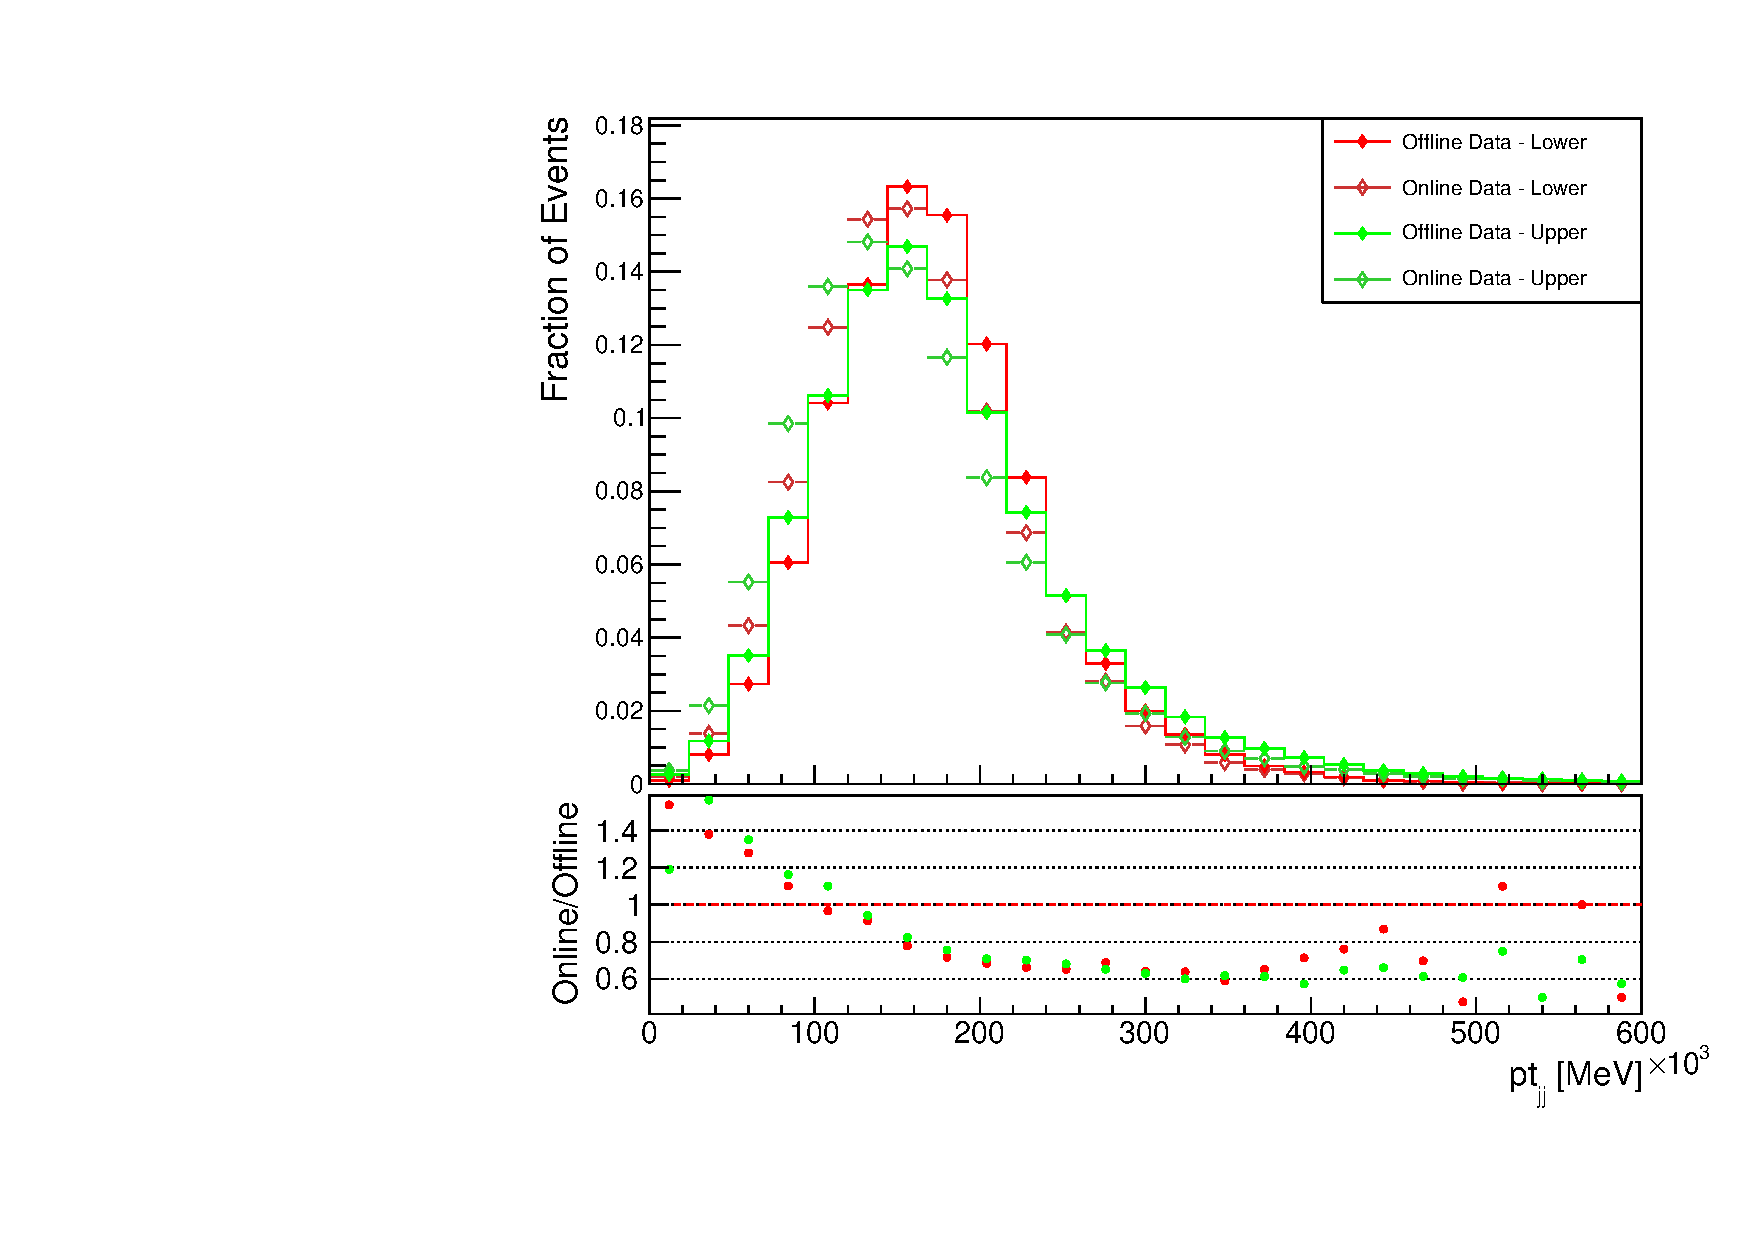
\includegraphics[width=1\linewidth]{ptjj_data_}
            \end{minipage}
            \quad
            \begin{minipage}[h]{0.48\linewidth}
                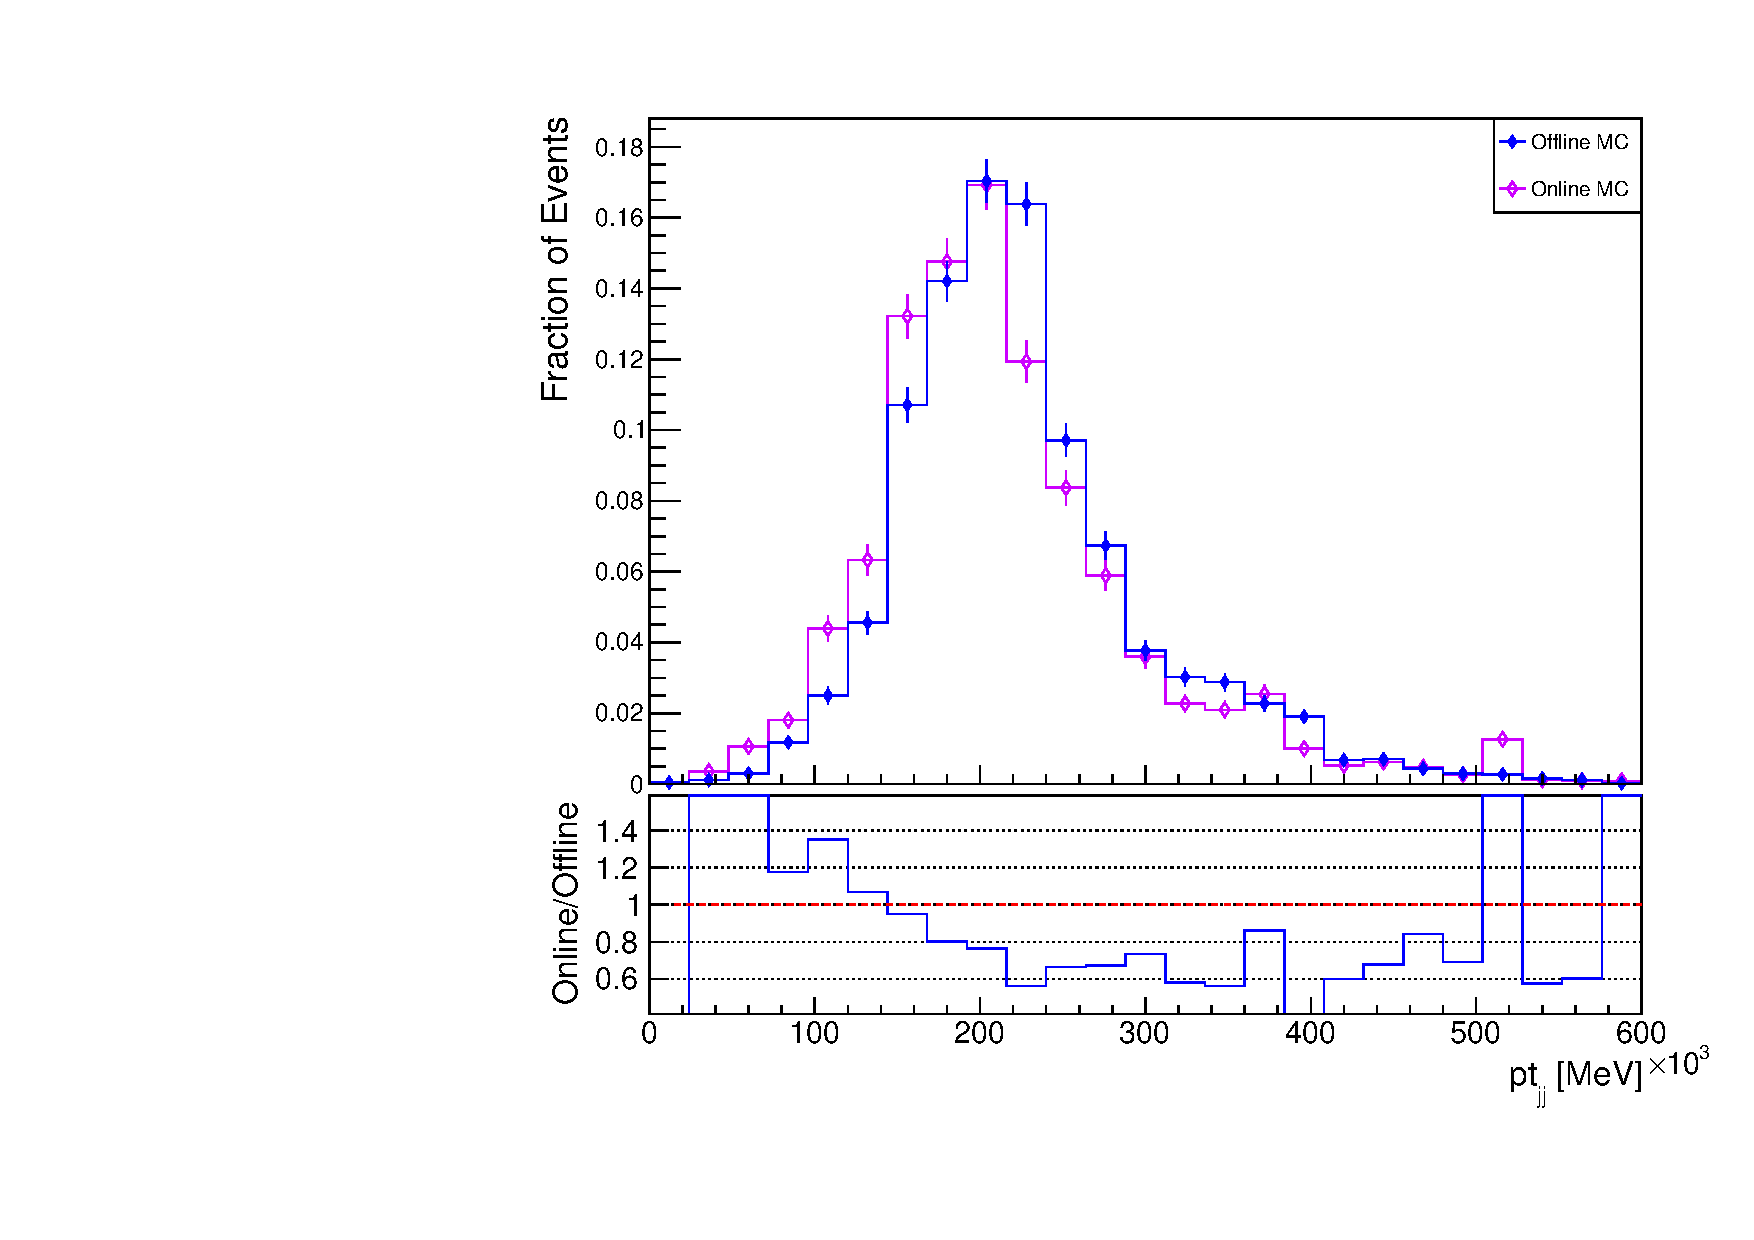
\includegraphics[width=1\linewidth]{ptjj_mc_}
            \end{minipage}
            \caption[Comparison of the \ptjj distribution of the \VBFHBB\ events for HLT and offline objects]{\ptjj distribution for the online and offline \VBFHBB\ events, with background events from data shown in the left panel and Monte-Carlo signal events in the right.}
        	\label{f:ptjj}
        \end{figure}

        \begin{figure}[h]
            \centering
            \begin{minipage}[h]{0.48\linewidth}
                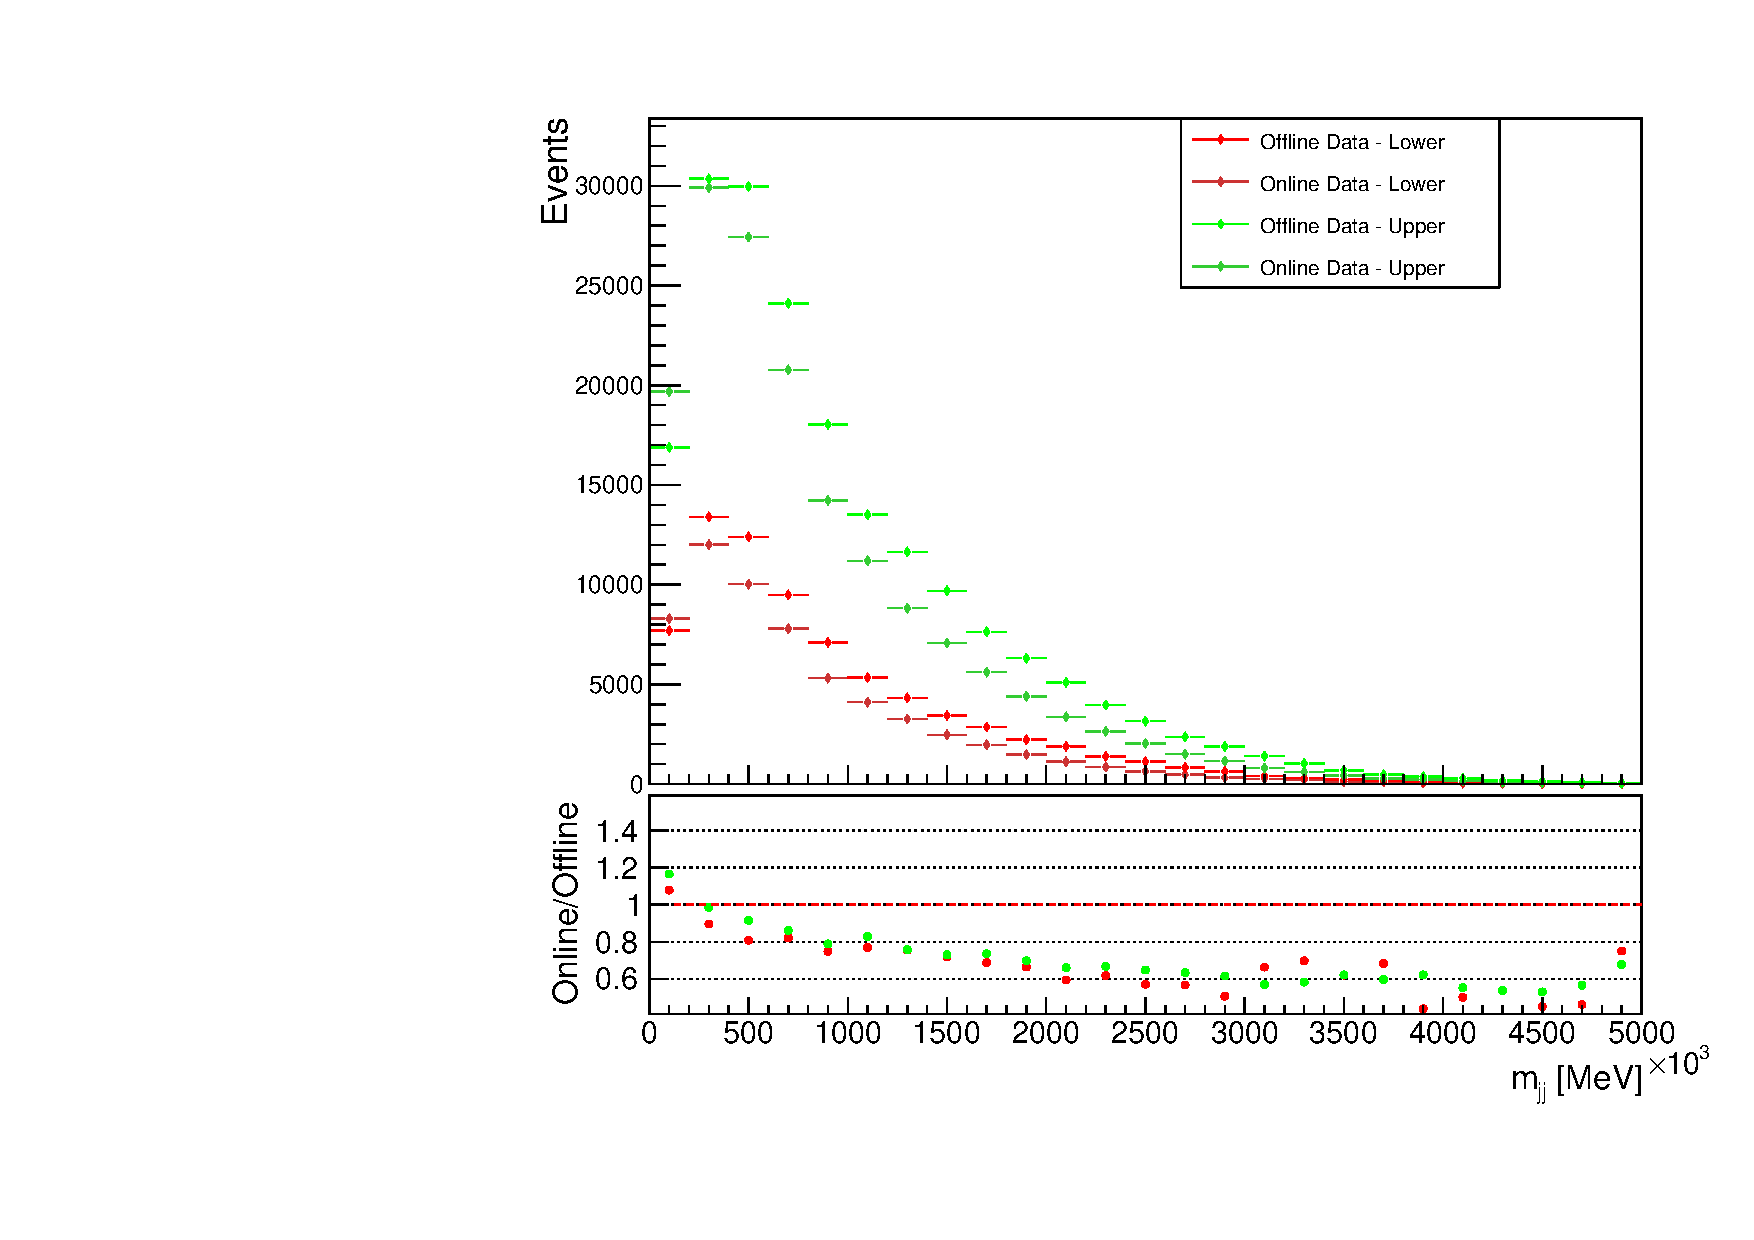
\includegraphics[width=1\linewidth]{mjj_data_}
            \end{minipage}
            \quad
            \begin{minipage}[h]{0.48\linewidth}
                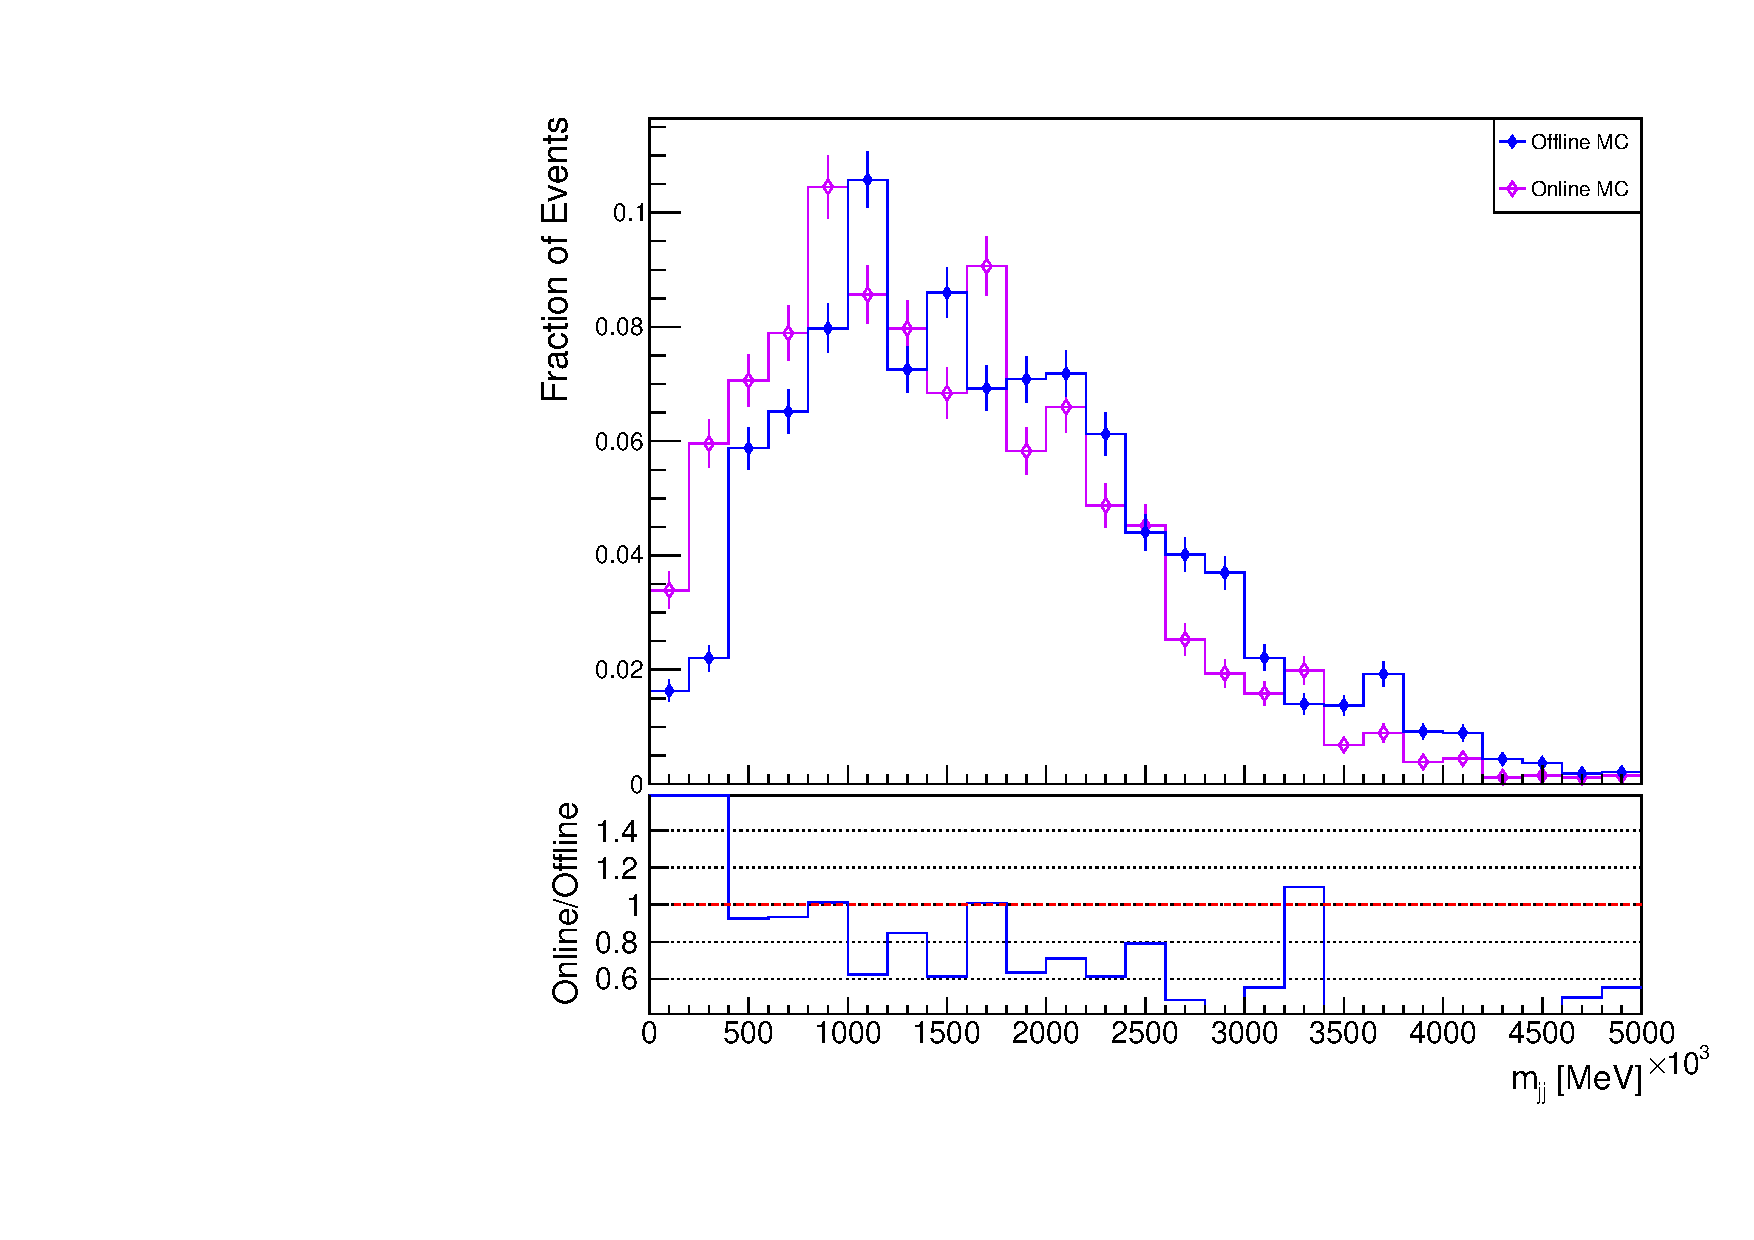
\includegraphics[width=1\linewidth]{mjj_mc_}
            \end{minipage}
            \caption[Comparison of the \mjj distribution of the \VBFHBB\ events for HLT and offline objects]{\mjj distribution for the online and offline \VBFHBB\ events, with background events from data shown in the left panel and Monte-Carlo signal events in the right.}
            \label{f:mjj}
        \end{figure}

        The \ptjj distributions shown in Figure \ref{f:ptjj} are similar to the plots of the leading non-\bjet\ shown in Figure \ref{f:ptj1}. The peak of the online distribution in the upper and lower background regions along with the signal region is shifted down in \ptjj in relation to the offline region. The overall shape of the distribution is consistent between the Monte-Carlo simulations and the data background regions, and the ratio plot shows similar characteristics to that in Figure~\ref{f:ptj1}, flattening off at an online/offline ratio value of $\sim0.7$. These features are replicated in the \mjj plot in Figure \ref{f:mjj}: similar distribution shapes for upper background, lower background and signal, increased numbers of online events compared to offline events at low \mjj (which corresponds to low non-\bjet\ $p_\text{T}$), the online/offline ratio flattening off to a value of $\sim0.7$. These features, as described in Section \ref{k:jets}, could be explained by the differences observed at low \pt regions for non-\bjets\ in Section \ref{OP:leadingnonb}. Overall the performance of online is comparable to offline, so these variables may be used to train a BDT and perform any further analysis using TLA methodologies.

        \begin{figure}[h]
            \centering
            \begin{minipage}[h]{0.48\linewidth}
                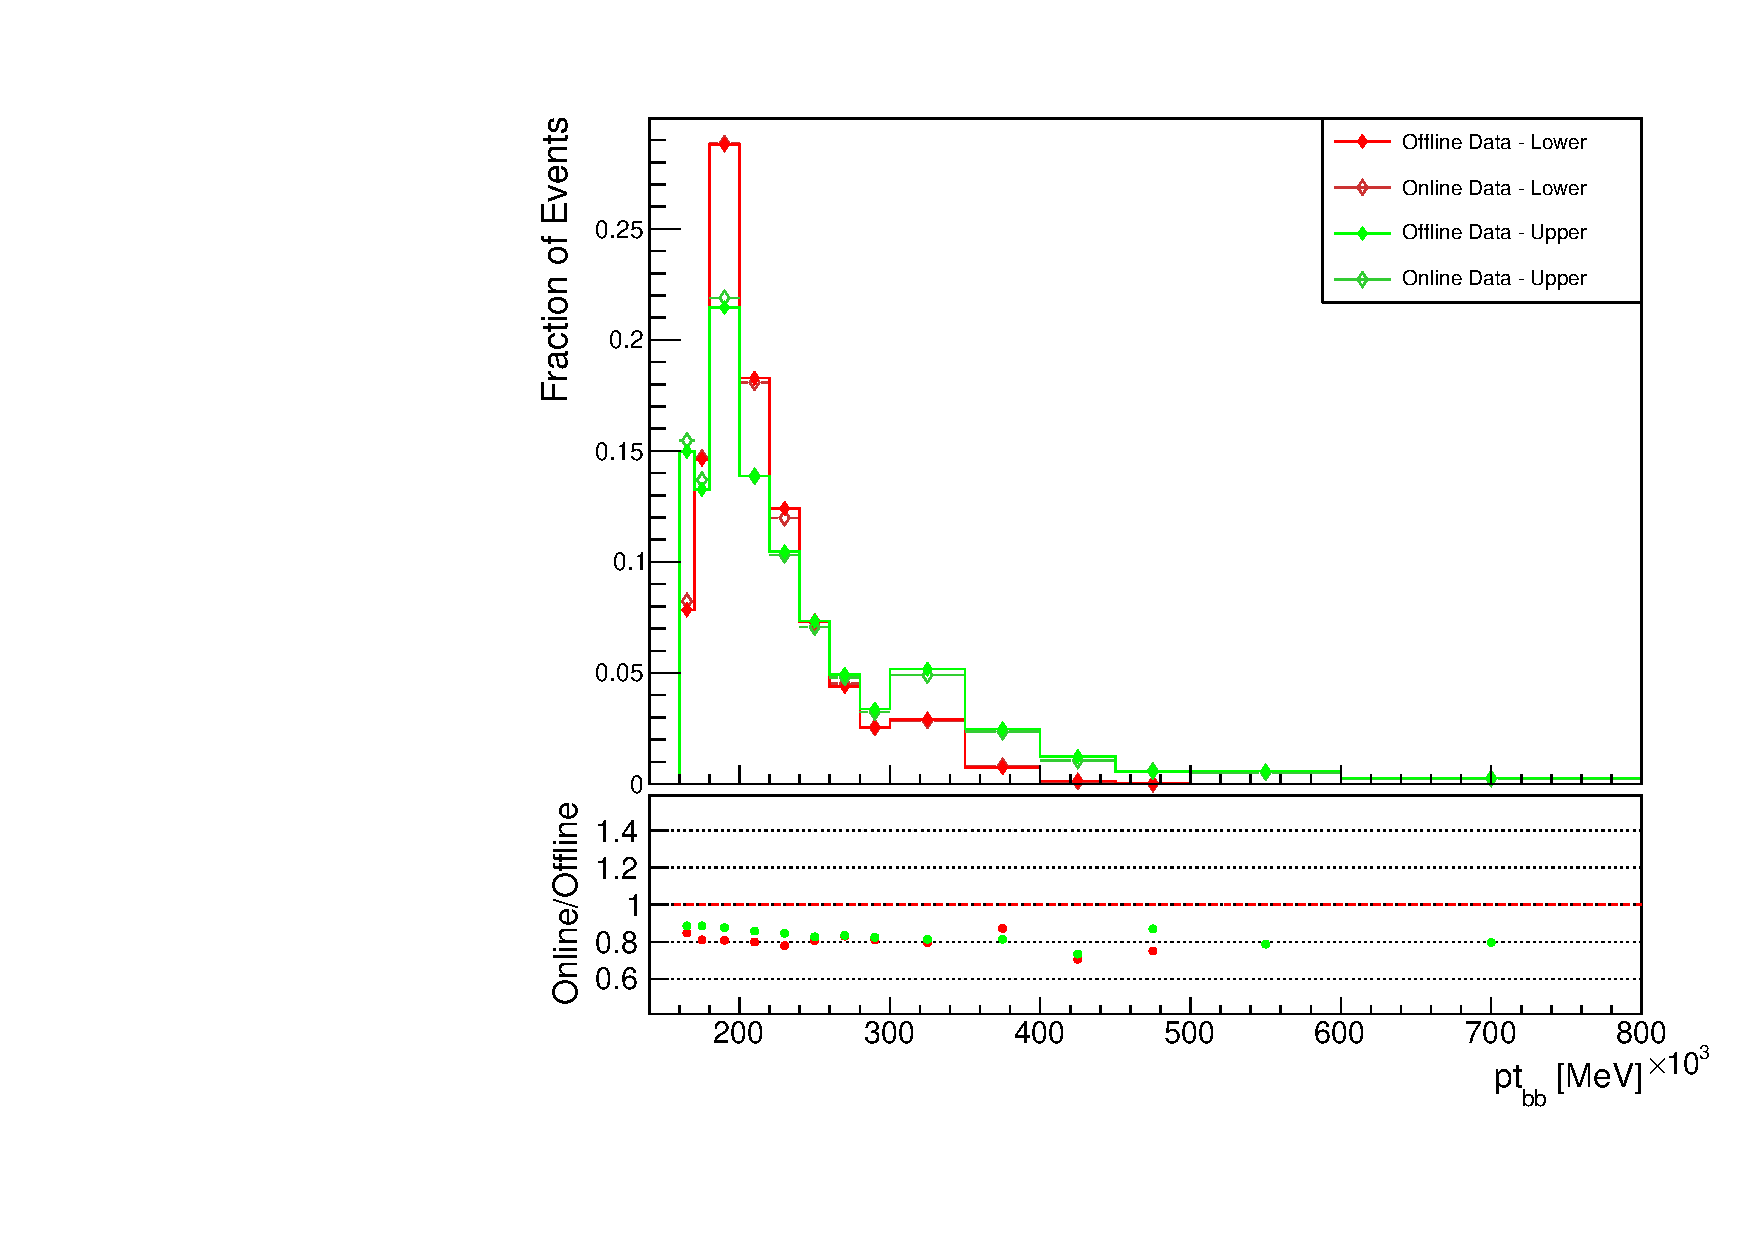
\includegraphics[width=1\linewidth]{ptbb_data_}
            \end{minipage}
            \quad
            \begin{minipage}[h]{0.48\linewidth}
                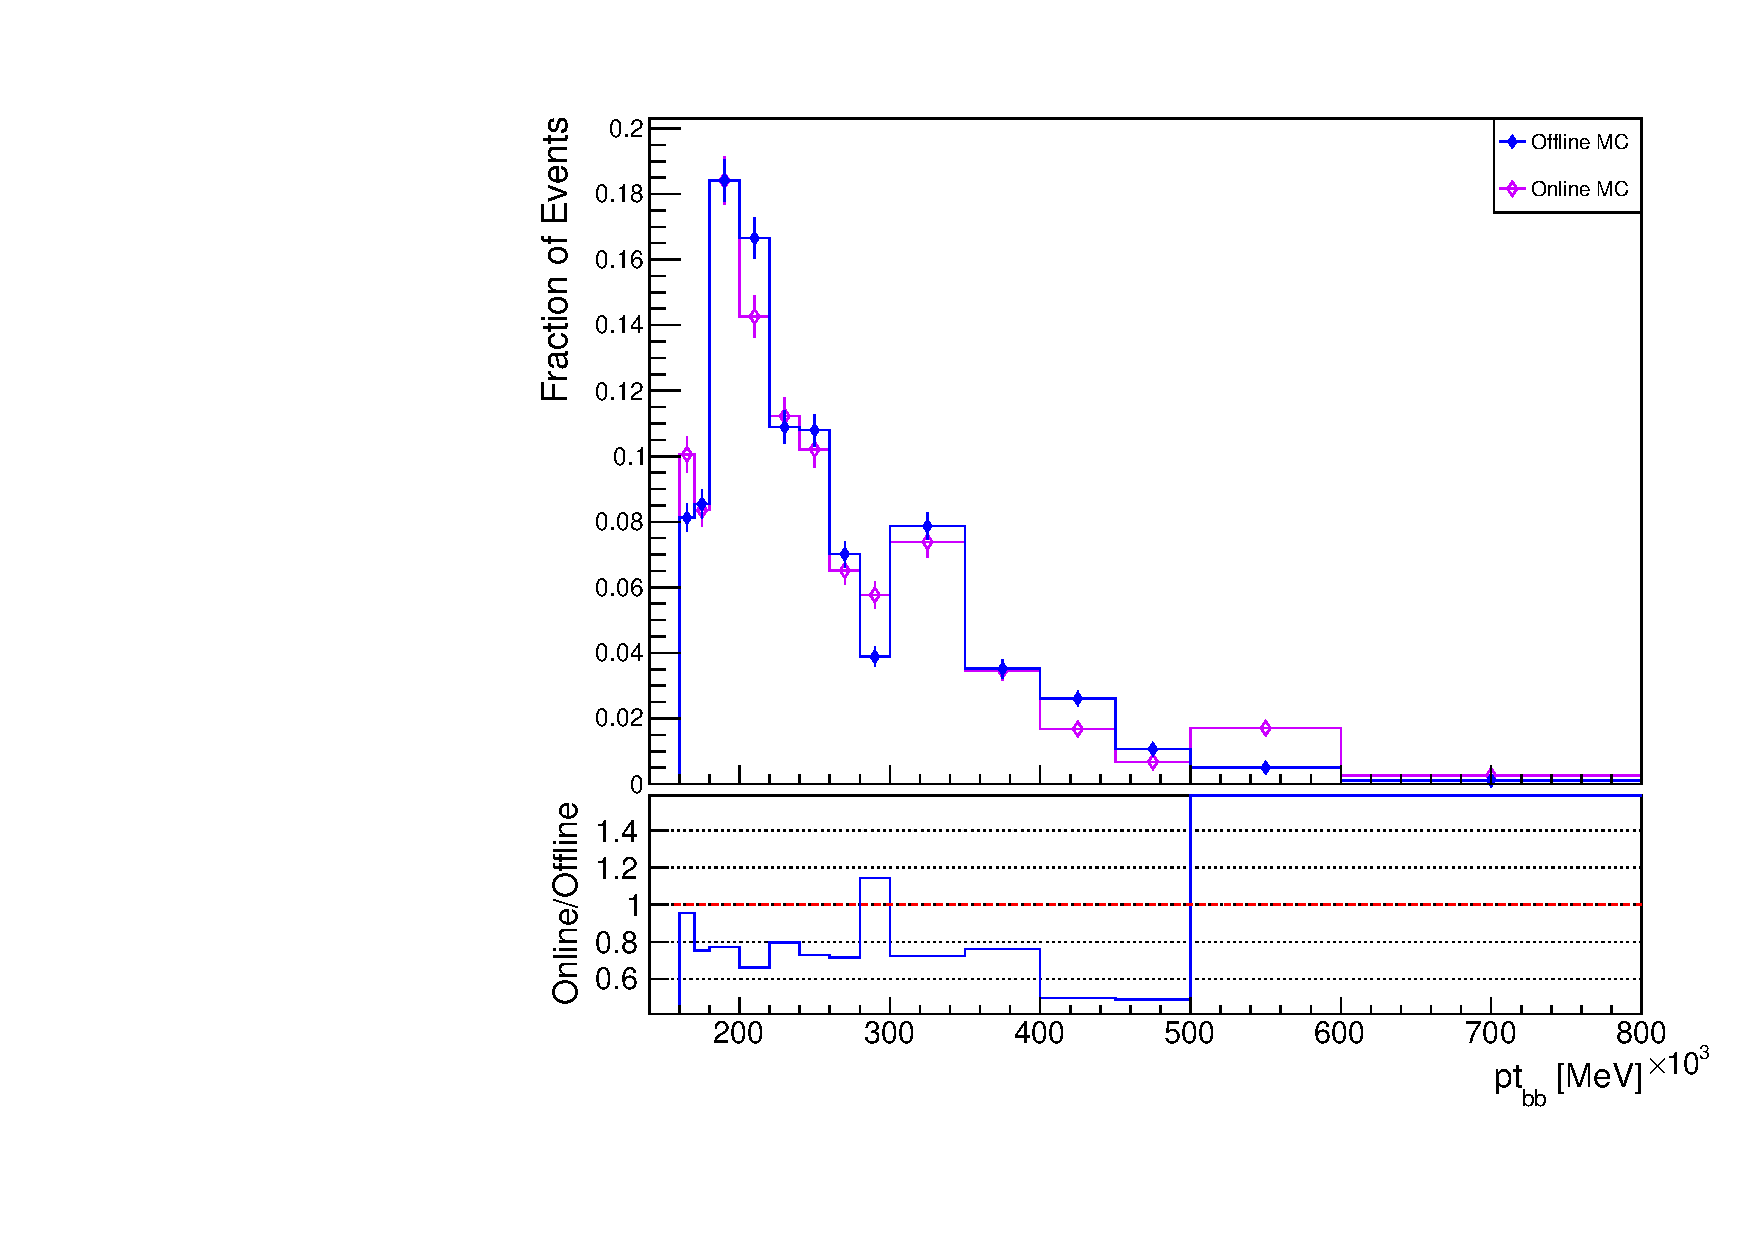
\includegraphics[width=1\linewidth]{ptbb_mc_}
            \end{minipage}
            \caption[Comparison of the \ptbb distribution of the \VBFHBB\ events for HLT and offline objects]{\ptbb distribution for the online and offline \VBFHBB\ events, with background events from data shown in the left panel and Monte-Carlo signal events in the right.}
            \label{f:ptbb}
        \end{figure}

        The plots of \ptbb in Figure \ref{f:ptbb} show excellent agreement between the online and offline objects. The ratio in the left panel of the Figure shows a flat line around $\sim0.8$, in strong agreement with the reduction in event count shown in Figure \ref{f:cutflowD}. This agreement with the expected decrease is also shown in the signal events, which agree with Figure \ref{f:cutflowMC}. For $p_{\text{T}bb}$, the same behaviour is seen for online and offline jets, indicating there is no additional problems for applying a TLA beyond the rate reduction.

        \begin{figure}[h]
            \centering
            \begin{minipage}[h]{0.48\linewidth}
                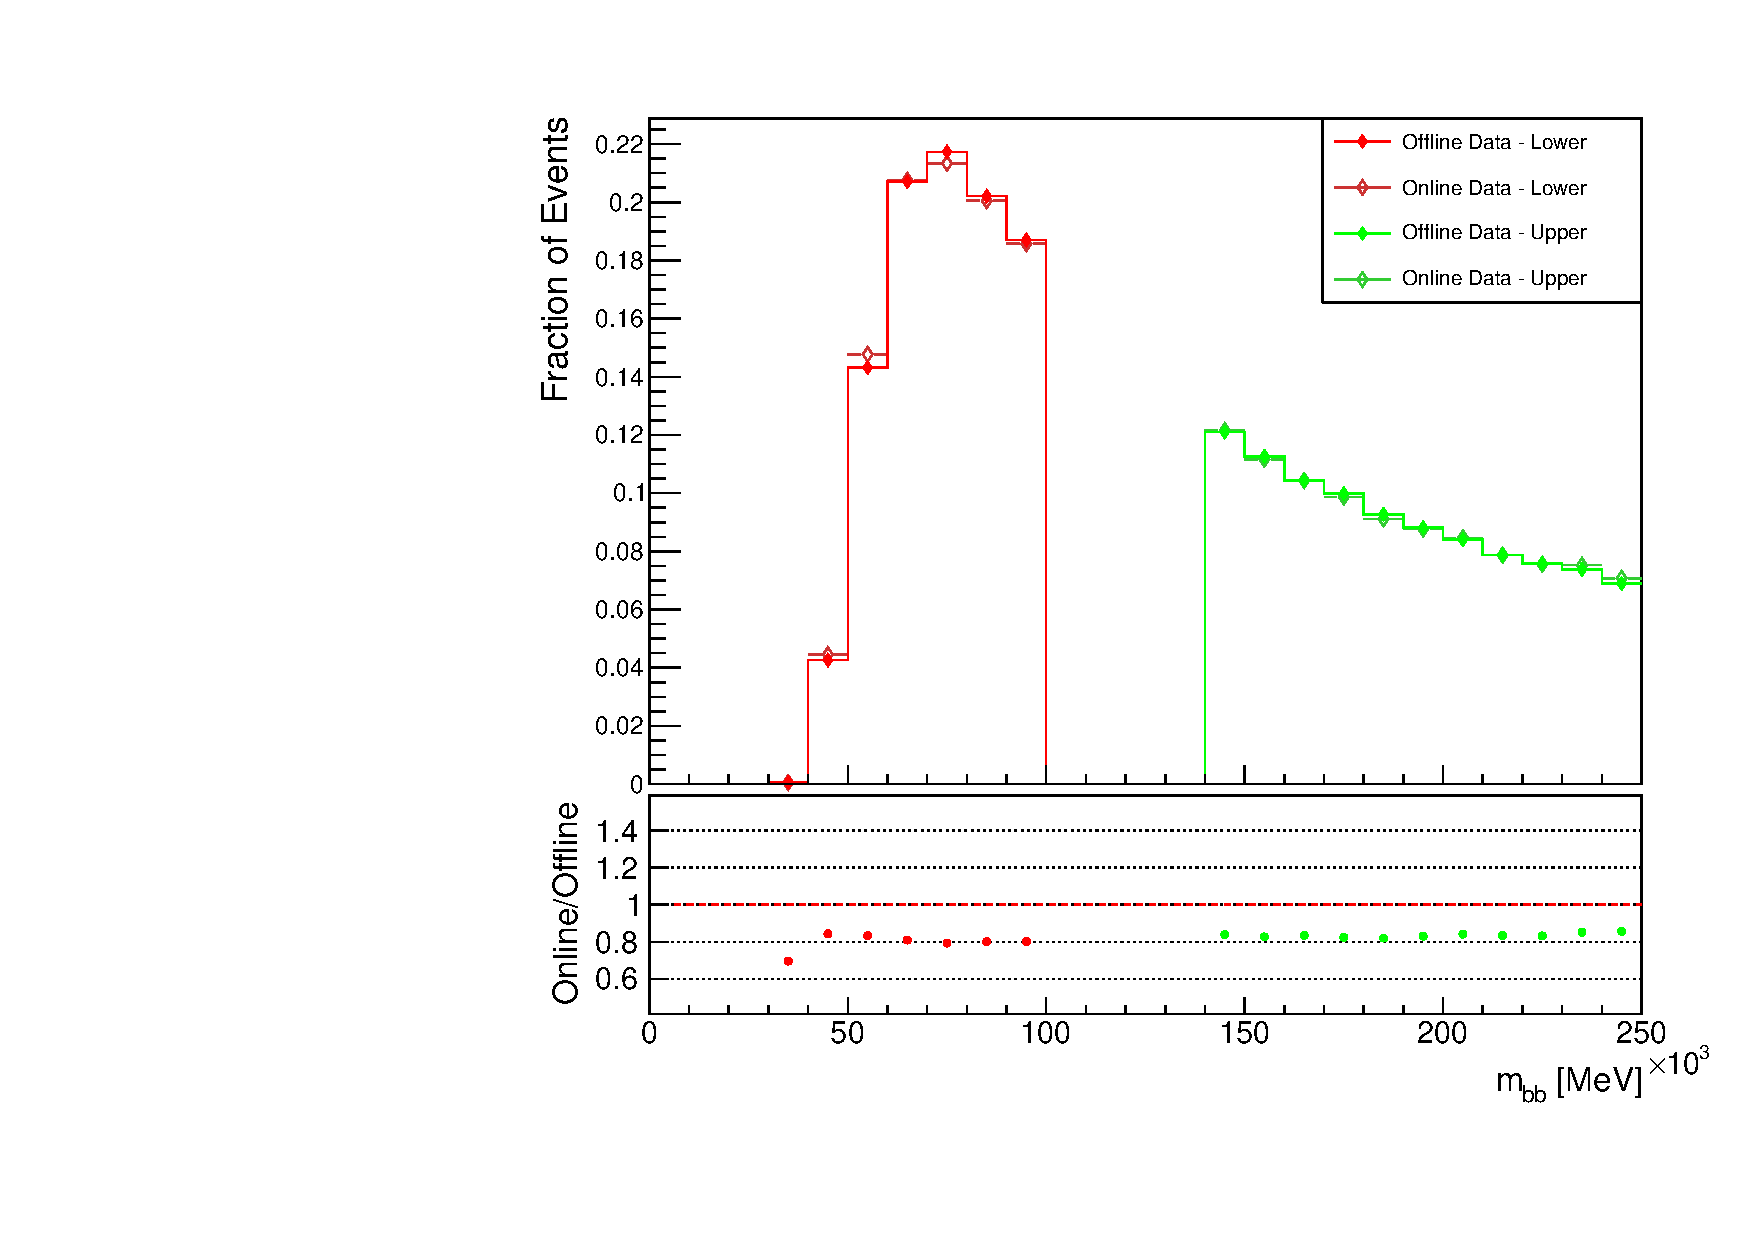
\includegraphics[width=1\linewidth]{mbb_data_}
            \end{minipage}
            \quad
            \begin{minipage}[h]{0.48\linewidth}
                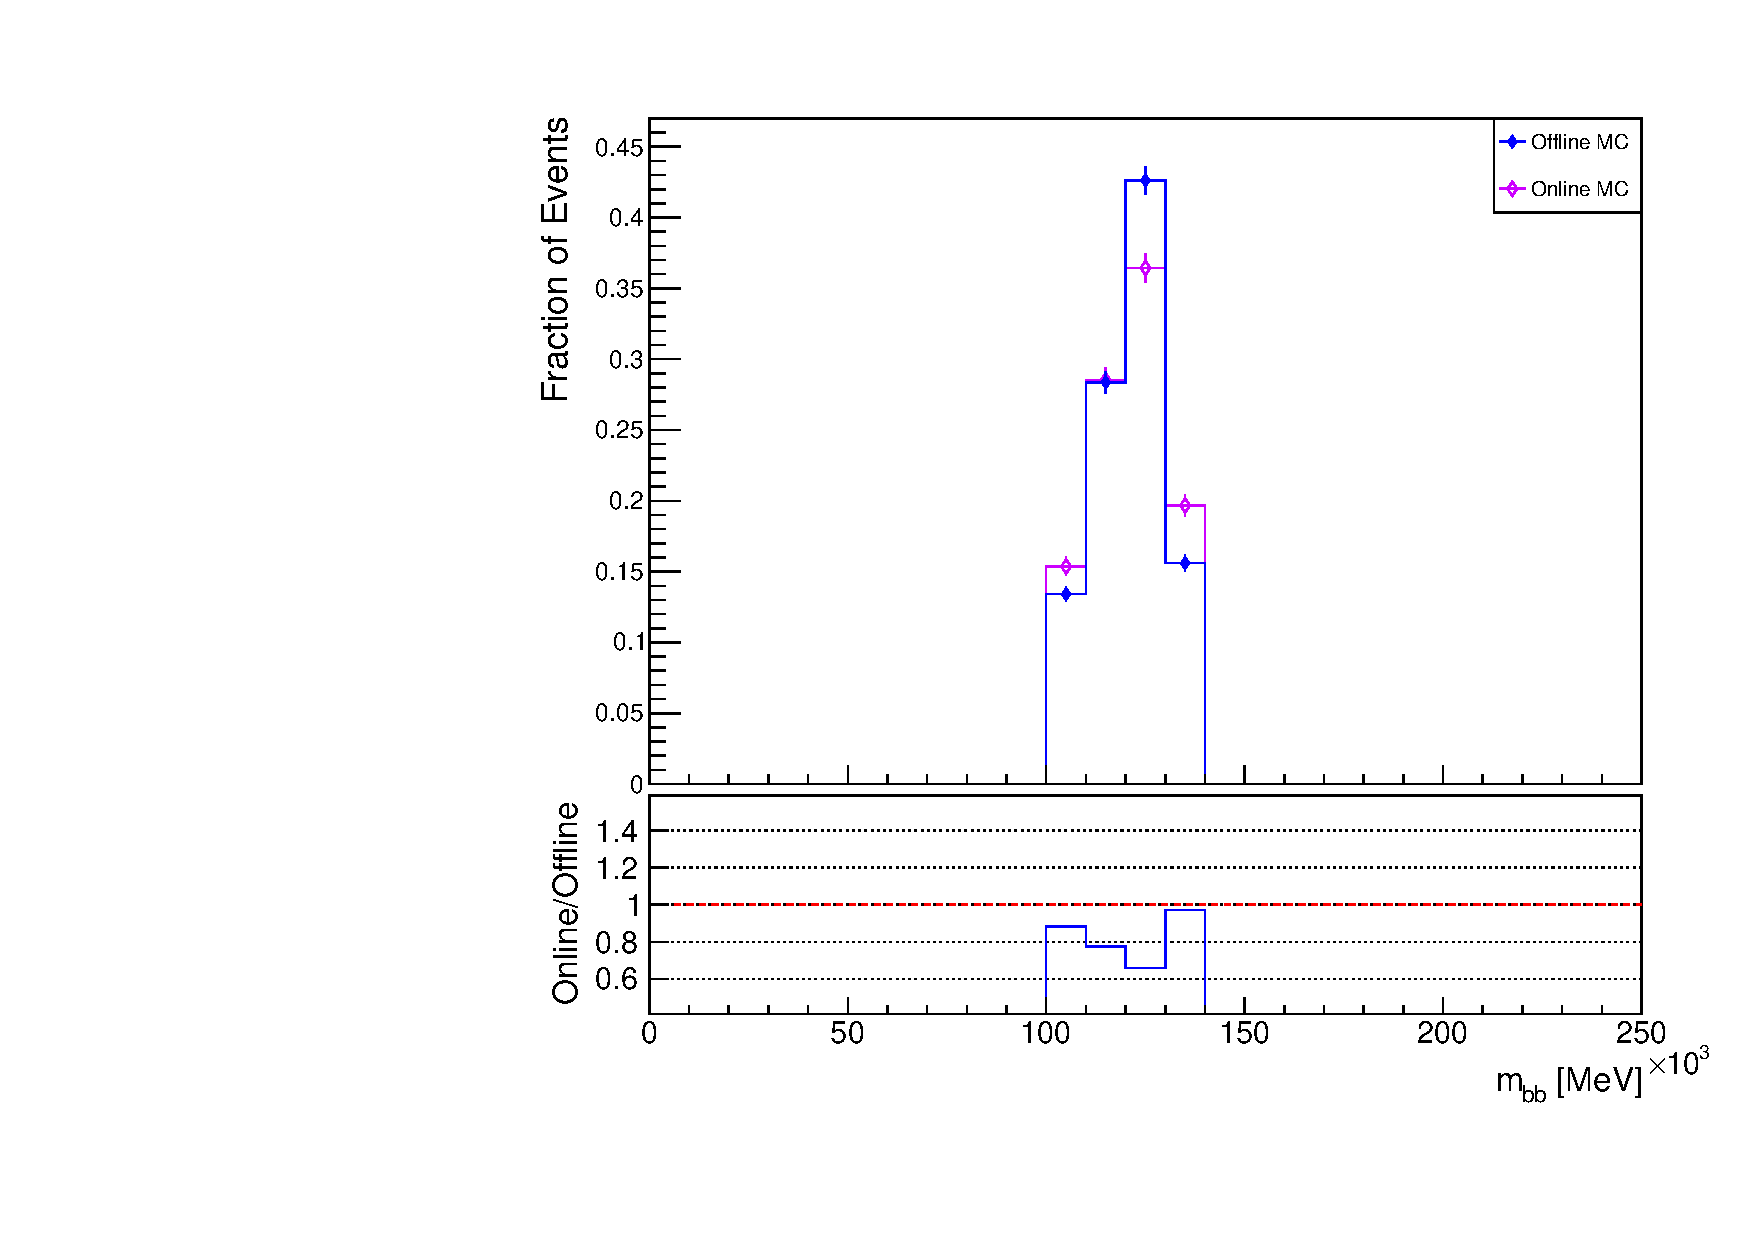
\includegraphics[width=1\linewidth]{mbb_mc_}
            \end{minipage}
            \caption[Comparison of the \mbb distribution of the \VBFHBB\ events for HLT and offline objects]{\mbb distribution for the online and offline \VBFHBB\ events, with background events from data shown in the left panel and Monte-Carlo signal events in the right.}
            \label{f:mbb}
        \end{figure}

        The \mbb plot in Figure \ref{f:mbb} for the background data events shows the online and offline analysis to be in good agreement. The online/offline ratio is a flat line at $\sim0.8$ as expected from the ratio plot in Figure \ref{f:cutflowD}. The behaviour of the upper and lower background region suggests a consistently decreasing function for \mbb beyond the peak at \pt$\sim80$~GeV, and look to link up across the signal region. The signal region is less clear than the background data, but suggests a ratio value of $\sim0.8$ and shows comparable behaviour for the online and offline jets. As for the other kinematic quantities in this section, the variables derived from the $b\bar{b}$ pair look to behave consistently for online and offline and so could be used in a TLA.
\section{BDT Input Variables}

    As discussed in Section \ref{es:as}, the full BDT analysis of the \VBFHBB\ search described in Appendix \ref{a:bdt} was not performed for this dissertation. Given this is a critical component of the full Higgs search\cite{VBFHbb8tev} in \VBFHBB, the performance of select BDT variables is explored for the signal and background regions described in Table \ref{t:signalback}. The variables \mjj and \ptjj covered in the previous section are both BDT training variables.

    This section covers $\eta^*$, given by

    \begin{equation}
    \eta^* = \frac{1}{2}(|\eta_{j1}| + |\eta_{j2}| - |\eta_{b1}| - |\eta_{b2}|),
    \end{equation}

    which is plotted in Figure \ref{f:etastar} for the online and offline events, and the $p_{\text{T} balance}$, given by

    \begin{equation}
        p_{\text{T} balance} = \frac{\vec{p_{\text{T}j1}} + \vec{p_{\text{T}j2}} + \vec{p_{\text{T}b1}} + \vec{p_{\text{T}b2}}}{p_{\text{T}j1} + p_{\text{T}j2} + p_{\text{T}b1} + p_{\text{T}b2}},
    \end{equation}

    which is shown in Figure \ref{f:ptbalance}.

    \begin{figure}[h]
        \centering
        \begin{minipage}[h]{0.48\linewidth}
            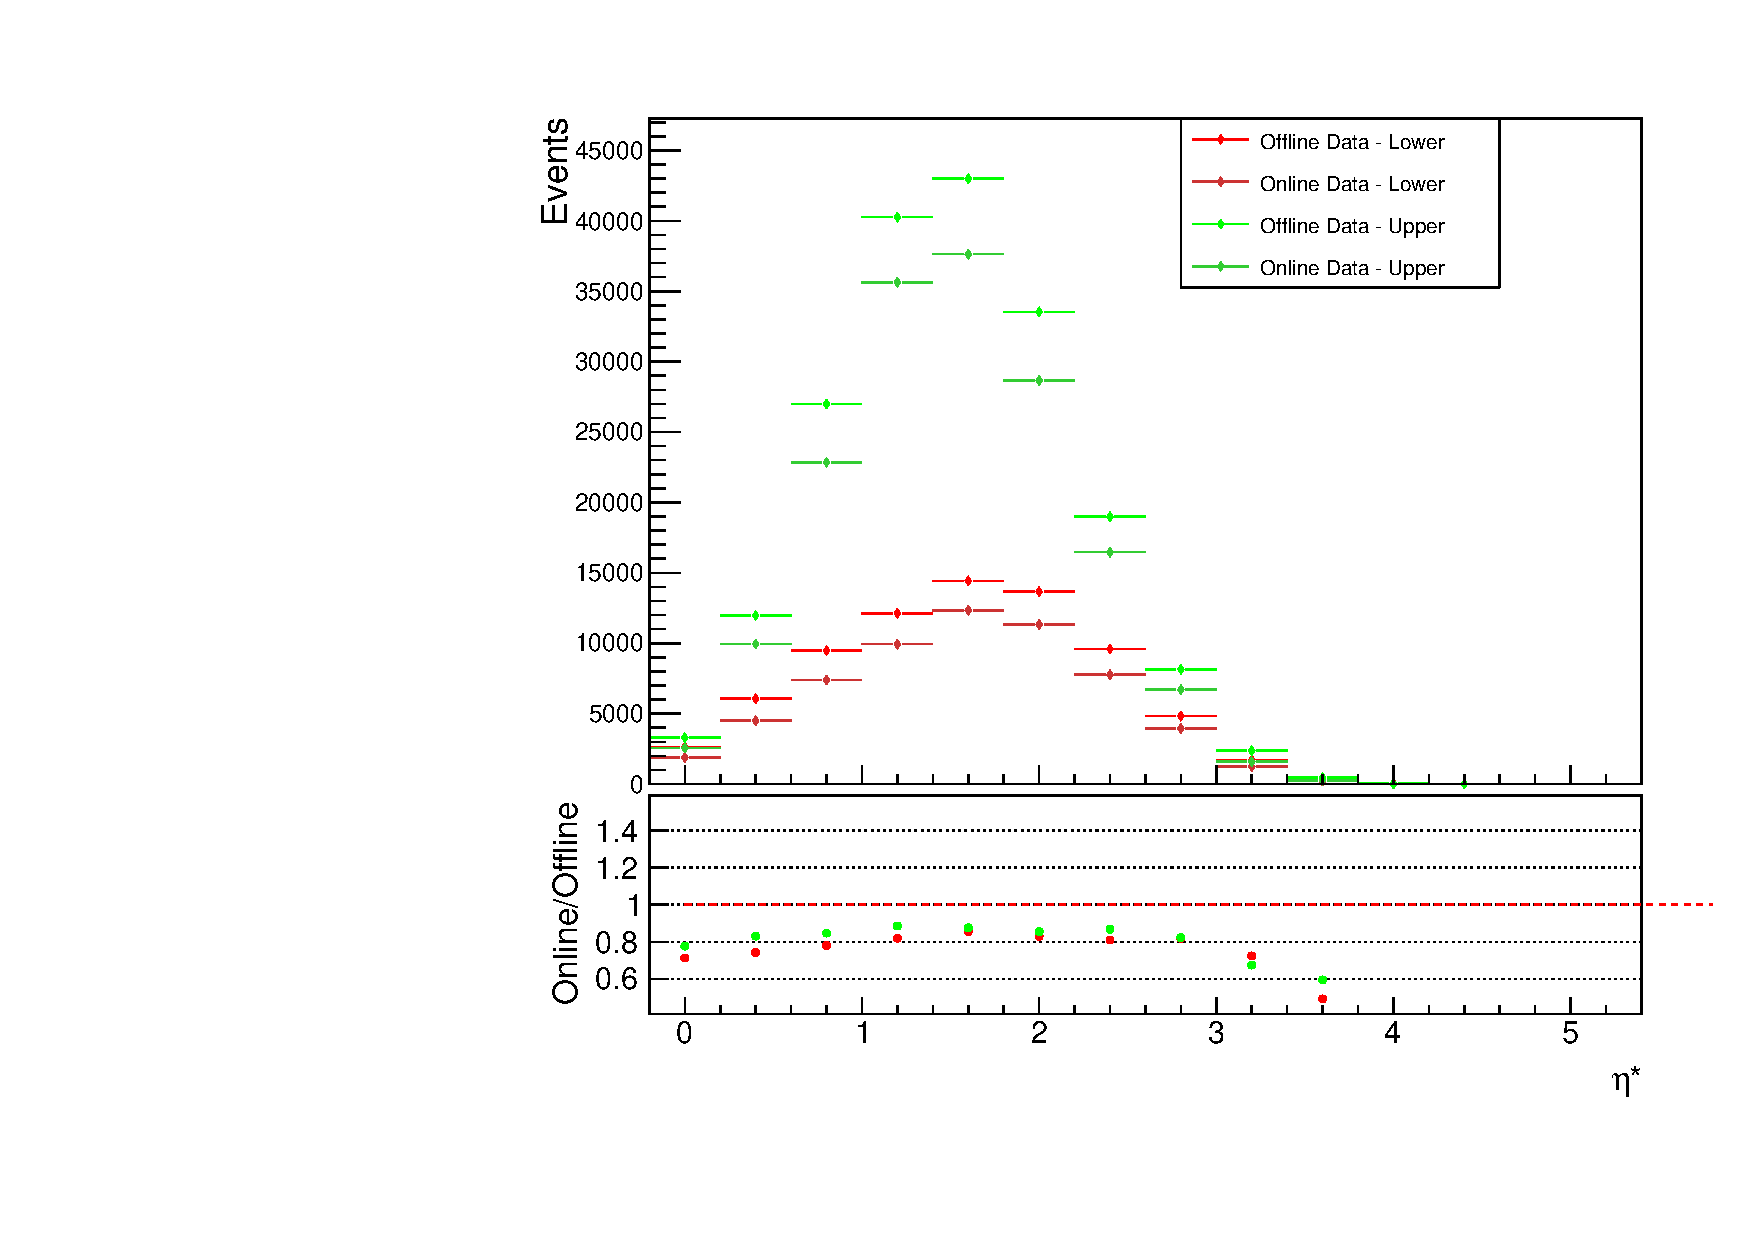
\includegraphics[width=1\linewidth]{etastar_data_}
        \end{minipage}
        \quad
        \begin{minipage}[h]{0.48\linewidth}
            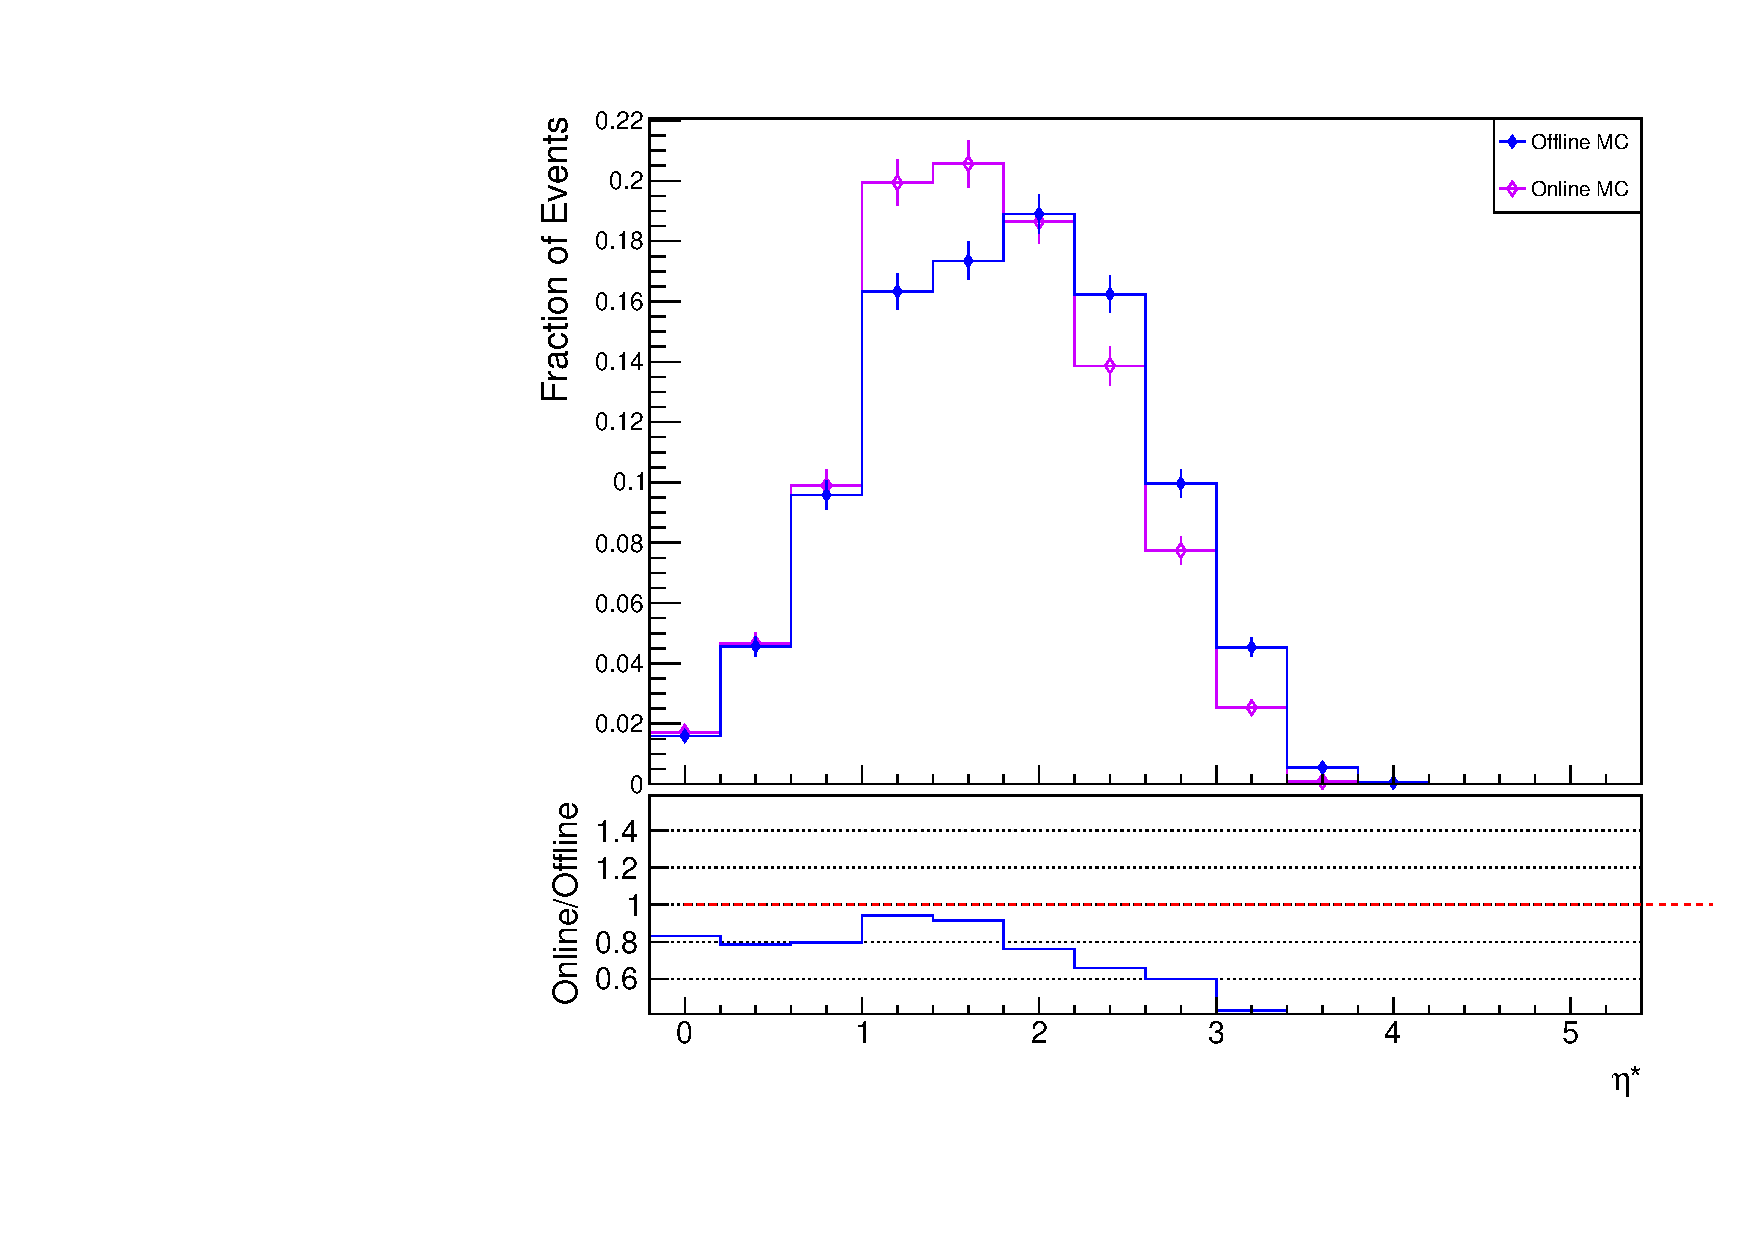
\includegraphics[width=1\linewidth]{etastar_mc_}
        \end{minipage}
        \caption[Comparison of the $\eta^*$ distribution of the \VBFHBB\ events for HLT and offline objects]{$\eta^*$ distribution for the online and offline \VBFHBB\ events, with background events from data shown in the left panel and Monte-Carlo signal events in the right.}
        \label{f:etastar}
    \end{figure}

    \begin{figure}[h]
        \centering
        \begin{minipage}[h]{0.48\linewidth}
            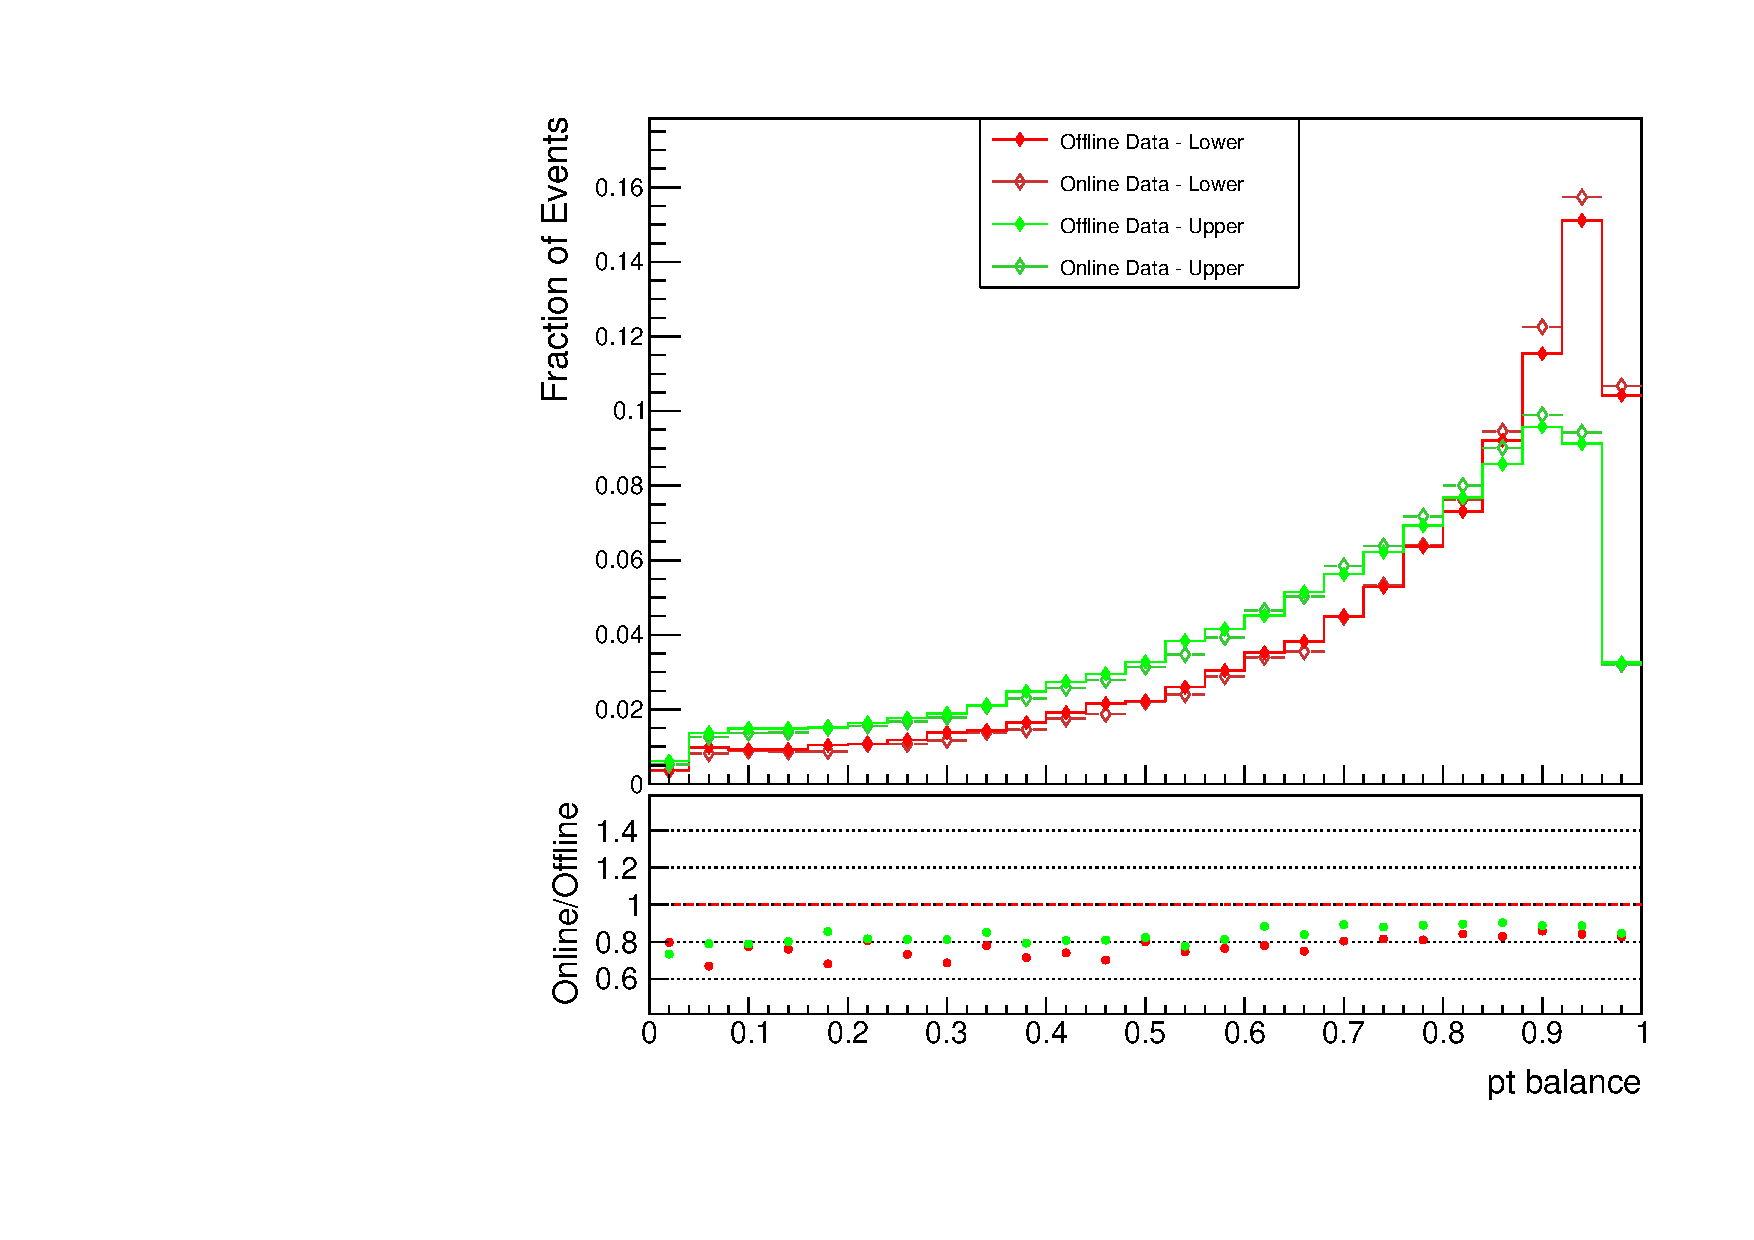
\includegraphics[width=1\linewidth]{ptbalance_data_}
        \end{minipage}
        \quad
        \begin{minipage}[h]{0.48\linewidth}
            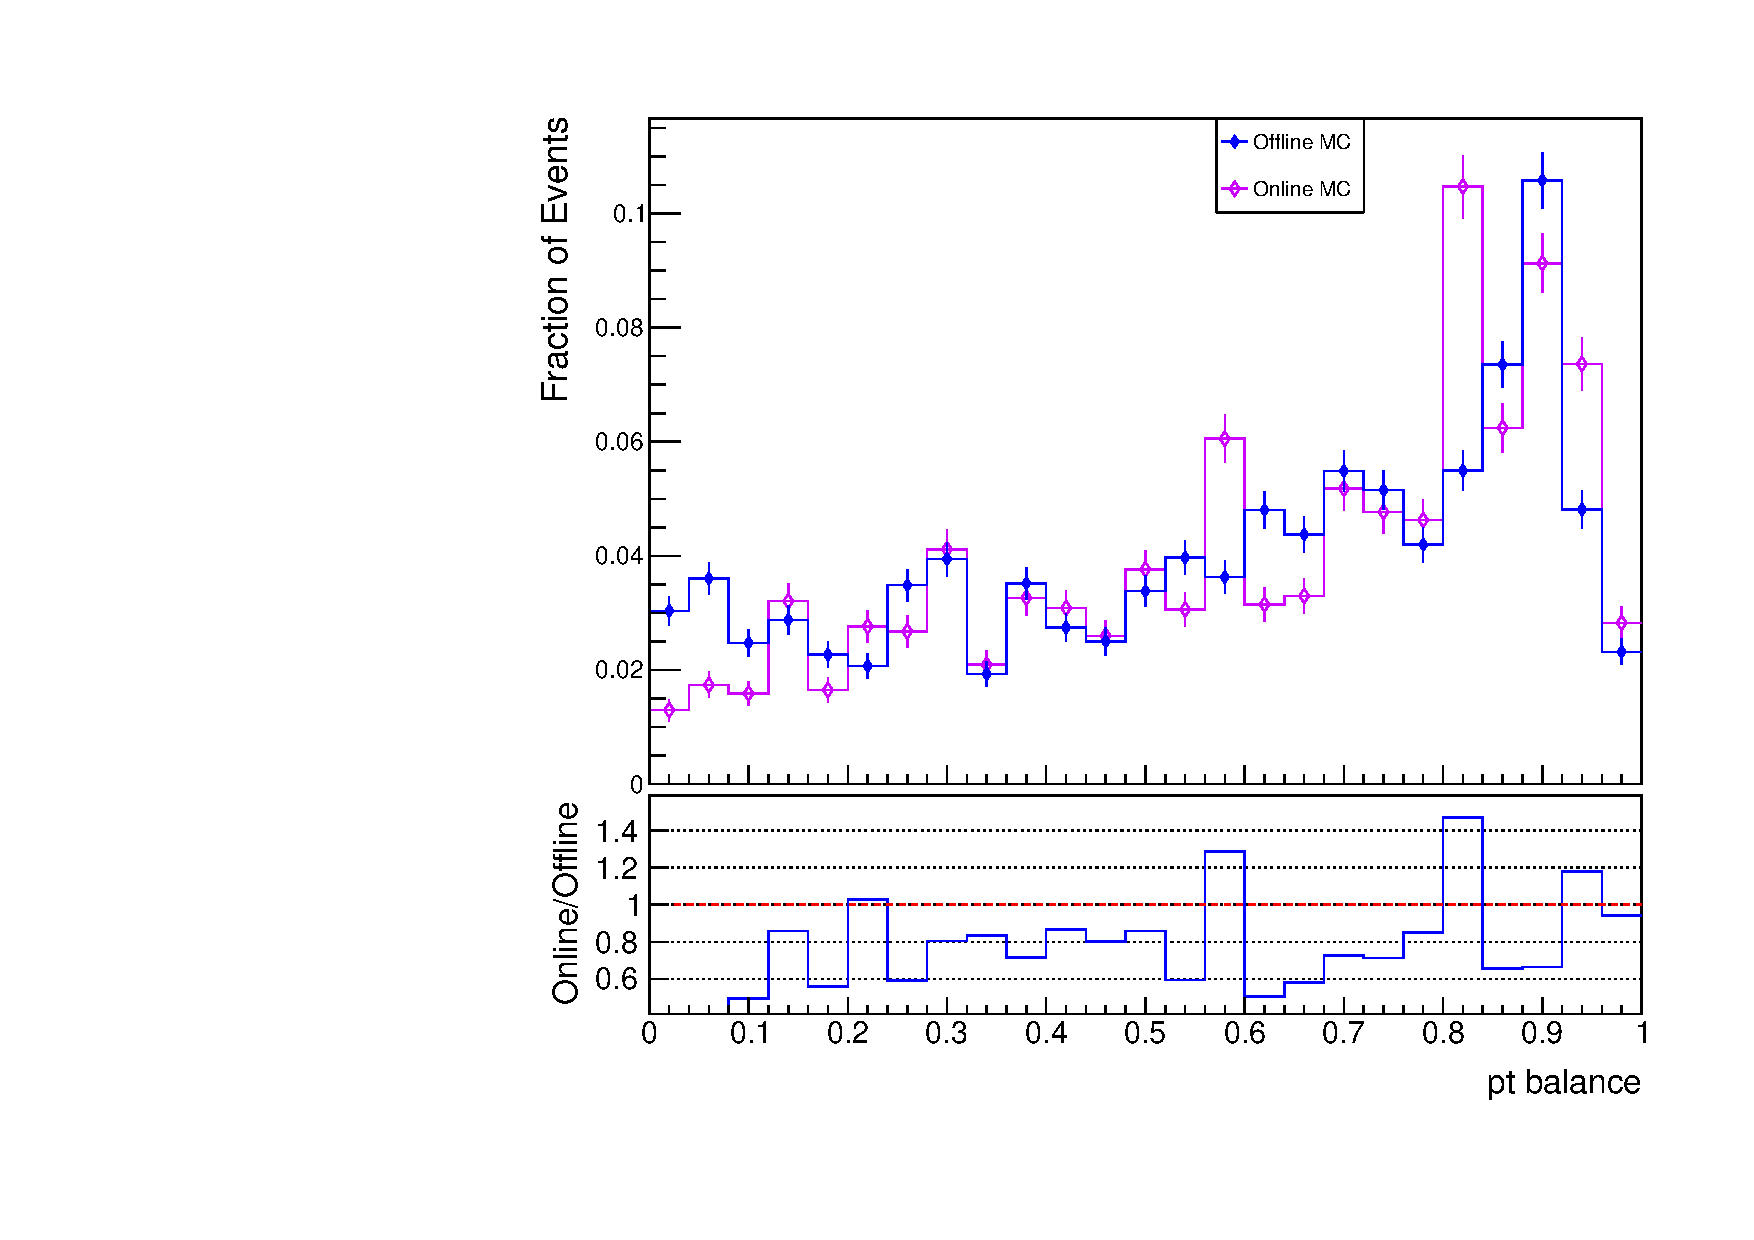
\includegraphics[width=1\linewidth]{ptbalance_mc_}
        \end{minipage}
        \caption[Comparison of the $p_{\text{T} balance}$ distribution of the \VBFHBB\ events for HLT and offline objects]{$p_{\text{T} balance}$ distribution for the online and offline \VBFHBB\ events, with background events from data shown in the left panel and Monte-Carlo signal events in the right.}
        \label{f:ptbalance}
    \end{figure}

    These variables behave in a consistent fashion as to the other \VBFHBB\ kinematic quantities covered in this section. For the lower background, upper background and signal sectors the shapes of the online and offline curves are comparable. The relative ratio of the online to the offline events is $\sim0.8$, as covered in Section \ref{k:cutflow} and shown clearly by the ratio plots in the left panels of Figures \ref{f:etastar} and \ref{f:ptbalance}. The plots for the Monte-Carlo signal are less clear, but show a rough $20\%$ decrease in online events compared to offline, and in general the upper background region performs better than the lower region.

    Given the behaviour of the online and offline BDT quantities derived from the \VBFHBB\ event is similar, the trigger-level objects should perform comparably to the offline objects, and as such can be used in the training of a \VBFHBB\ BDT.
    \section{Summary}

    This chapter presents analysis and comparison of the \VBFHBB\ events obtained using trigger-level objects and offline reconstructions in data and Monte-Carlo simulation. The cutflows of the analysis for Monte-Carlo online, Monte-Carlo offline, data online and data offline were studied, and found to show online analysis produced $\sim82\%$ of the statistics of offline analysis for Monte-Carlo simulations, and $\sim84\%$ for data. These results are the overall decrease, the step by step changes of the cutflow were not predicted by the results from Chapter \ref{c:OP}. Section \ref{k:cutflow} contains discussion of some possible causes, and they could also be the result of some coding bugs in the analysis.

    With this reduction of event yield for a given analysis sample, the increased trigger rates permitted when applying TLA will result in an increased final event count. For current rate increases in TLA analyses \cite{tla}, this would amount to an increase of $\sim66\%$ in the final number of events. This estimate of the possible increase does not consider any limitations on the rate that may result from increased computational demands on either processing or TLA object byte size.

    To confirm that the TLA analysis would be possible with the trigger-level objects, the component jets, kinematic properties of the \VBFHBB\ event and select BDT training variables were investigated. These cases showed consistent behaviour between the online and offline objects in both background data and signal Monte-Carlo simulation, while showing the online rate decrease calculated from the cutflows.

    These results suggest a full study of \VBFHBB\ analysis is a feasible proposal. Use of TLA could increase the output rate of the triggers to statistically significant levels and the objects produced will behave during analysis in a consistent fashion to the offline objects.
\endinput
